\documentclass[aspectratio=169]{beamer}

%
% preamble file
%

% \usepackage[english]{babel}
\usepackage{amsmath}
\usepackage{color}
% \usepackage{minted}
\usepackage{hyperref}
\usepackage{multicol}
% \usepackage{tabularx}
\usepackage{tikz}

% % only inline todonotes work
% \usepackage{xkeyval}
% \usepackage[textsize=small]{todonotes}
% \presetkeys{todonotes}{inline}{}

\usetikzlibrary{shapes,arrows,positioning,shadows}

% % no nav buttons
% \usenavigationsymbolstemplate{}

\newcommand{\bftt}[1]{\textbf{\texttt{#1}}}
\newcommand{\comment}[1]{{\color[HTML]{008080}\textit{\textbf{\texttt{#1}}}}}
\newcommand{\cmd}[1]{{\color[HTML]{008000}\bftt{#1}}}
\newcommand{\bs}{\char`\\}
\newcommand{\cmdbs}[1]{\cmd{\bs#1}}
\newcommand{\lcb}{\char '173}
\newcommand{\rcb}{\char '175}
\newcommand{\cmdbegin}[1]{\cmdbs{begin\lcb}\bftt{#1}\cmd{\rcb}}
\newcommand{\cmdend}[1]{\cmdbs{end\lcb}\bftt{#1}\cmd{\rcb}}

\newcommand{\wllogo}{\textbf{Overleaf}}

% this is where the example source files are loaded from
% do not include a trailing slash
% \newcommand{\fileuri}{https://raw.github.com/jdleesmiller/latex-course/master/en}
\newcommand{\fileuri}{https://raw.github.com/jonaswagner2826/CSSC_F22_LatexWorkshop/master/templates}


\newcommand{\wlserver}{https://www.overleaf.com}
\newcommand{\wlnewdoc}[1]{\wlserver/docs?snip\_uri=\fileuri/#1\&splash=none}

\def\tikzname{Ti\emph{k}Z}

% from http://tex.stackexchange.com/questions/5226/keyboard-font-for-latex
\newcommand*\keystroke[1]{%
  \tikz[baseline=(key.base)]
    \node[%
      draw,
      fill=white,
      drop shadow={shadow xshift=0.25ex,shadow yshift=-0.25ex,fill=black,opacity=0.75},
      rectangle,
      rounded corners=2pt,
      inner sep=1pt,
      line width=0.5pt,
      font=\scriptsize\sffamily
    ](key) {#1\strut}
  ;
}
\newcommand{\keystrokebftt}[1]{\keystroke{\bftt{#1}}}

% % stolen from minted.dtx
% \newenvironment{exampletwoup}
%   {\VerbatimEnvironment
%    \begin{VerbatimOut}{example.out}}
%   {\end{VerbatimOut}
%    \setlength{\parindent}{0pt}
%    \fbox{\begin{tabular}{l|l}
%    \begin{minipage}{0.55\linewidth}
%      \inputminted[fontsize=\small,resetmargins]{latex}{example.out}
%    \end{minipage} &
%    \begin{minipage}{0.35\linewidth}
%      \input{example.out}
%    \end{minipage}
%    \end{tabular}}}

% \newenvironment{exampletwouptiny}
%   {\VerbatimEnvironment
%    \begin{VerbatimOut}{example.out}}
%   {\end{VerbatimOut}
%    \setlength{\parindent}{0pt}
%    \fbox{\begin{tabular}{l|l}
%    \begin{minipage}{0.55\linewidth}
%      \inputminted[fontsize=\scriptsize,resetmargins]{latex}{example.out}
%    \end{minipage} &
%    \begin{minipage}{0.35\linewidth}
%      \setlength{\parskip}{6pt plus 1pt minus 1pt}%
%      \raggedright\scriptsize\input{example.out}
%    \end{minipage}
%    \end{tabular}}}

% \newenvironment{exampletwouptinynoframe}
%   {\VerbatimEnvironment
%    \begin{VerbatimOut}{example.out}}
%   {\end{VerbatimOut}
%    \setlength{\parindent}{0pt}
%    \begin{tabular}{l|l}
%    \begin{minipage}{0.55\linewidth}
%      \inputminted[fontsize=\scriptsize,resetmargins]{latex}{example.out}
%    \end{minipage} &
%    \begin{minipage}{0.35\linewidth}
%      \setlength{\parskip}{6pt plus 1pt minus 1pt}%
%      \raggedright\scriptsize\input{example.out}
%    \end{minipage}
%    \end{tabular}}

% \title{An Interactive Introduction to \LaTeX}
% \author{Dr John D. Lees-Miller}
% \titlegraphic{%
% \includegraphics[height=36pt]{overleaf}\\[1em]
% \includegraphics[height=24pt]{UoB-logo}
% }




\mode<presentation>

%Theme and Color of Presentation
\usetheme{CambridgeUS}
\usecolortheme{seahorse}
\useinnertheme{rectangles}

%Colors
% From https://www.utdallas.edu/brand/color-palette/
\definecolor{UTDorange}{RGB}{232,117,0}
\definecolor{UTDgreen}{RGB}{18,71,52}
\definecolor{UTDseafoam}{RGB}{95,244,183}

\setbeamercolor{palette primary}{bg=UTDorange,fg=white}
\setbeamercolor{palette secondary}{bg=UTDgreen,fg=white}
\setbeamercolor{palette tertiary}{bg=UTDorange,fg=white}
\setbeamercolor{palette quaternary}{bg=UTDorange,fg=white}
\setbeamercolor{frametitle}{fg=UTDgreen}
\setbeamercolor{structure}{fg=UTDgreen} % itemize, enumerate, etc
\setbeamercolor{subsection in head/foot}{bg=UTDgreen,fg=white}


%Additional Packages
\usepackage{physics}
\usepackage{listings}
\usepackage{verbatim}
\usepackage{graphicx}
\usepackage{physics}
\usepackage{setspace}
\usepackage{textpos}


%Additional Settings/Commands
\newcommand{\extraspace}{\vskip 0.5em}
\newcommand{\R}{\mathbb{R}}
\newcommand{\st}{\ | \ }
\newcommand{\eig}{\text{eig}\qty }

\AtBeginSection[]
{
	\begin{frame}
		\frametitle{Outline}
    \begin{multicols}{2}
      \tableofcontents[currentsection]
    \end{multicols}
	\end{frame}
}

%listing settings
\lstset{
  basicstyle=\scriptsize,
  stringstyle=\ttfamily,
  showlines=true
}

\title{CSSC Fall 2022 Workshop on Latex}
\author{Jonas Wagner}
\date{Fall 2022}

\begin{document}

%%%%%%%%%%%%%%%%%%%%%%%%%%%%%%%%%%%%%%%%%%%%%%%%%%%%%%%%%%%%%%%%%%%%%%%%%%%%%%%
%%%%%%%%%%%%%%%%%%%%%%%%%%%%%%%%%%%%%%%%%%%%%%%%%%%%%%%%%%%%%%%%%%%%%%%%%%%%%%%
%%%%%%%%%%%%%%%%%%%%%%%%%%%%%%%%%%%%%%%%%%%%%%%%%%%%%%%%%%%%%%%%%%%%%%%%%%%%%%%
\begin{frame}
    \titlepage
\end{frame}

\addtobeamertemplate{frametitle}{}{%
    \begin{textblock*}{100mm}(.85\textwidth,-1cm)
        \includegraphics[height=1cm]{figs/UT_Dallas_Logo}
    \end{textblock*}
}

%%%%%%%%%%%%%%%%%%%%%%%%%%%%%%%%%%%%%%%%%%%%%%%%%%%%%%%%%%%%%%%%%%%%%%%%%%%%%%%
% Introduction
%%%%%%%%%%%%%%%%%%%%%%%%%%%%%%%%%%%%%%%%%%%%%%%%%%%%%%%%%%%%%%%%%%%%%%%%%%%%%%%
\section{What is \LaTeX{}?}
%%%%%%%%%%%%%%%%%%%%%%%%%%%%%%%%%%%%%%%%%%%%%%%%%%%%%%%%%%%%%%%%%%%%%%%%%%%%%%%
\subsection{Introduction}
%%%%%%%%%%%%%%%%%%%%%%%%%%%%%%%%%%%%%%%%%%%%%%%%%%%%%%%%%%%%%%%%%%%%%%%%%%%%%%%

%%%%%%%%%%%%%%%%%%%%%%%%%%%%%%%%%%%%%%%%%%%%%%%%%%%%%%%%%%%%%%%%%%%%%%%%%%%%%%%
%%%%%%%%%%%%%%%%%%%%%%%%%%%%%%%%%%%%%%%%%%%%%%%%%%%%%%%%%%%%%%%%%%%%%%%%%%%%%%%
%%%%%%%%%%%%%%%%%%%%%%%%%%%%%%%%%%%%%%%%%%%%%%%%%%%%%%%%%%%%%%%%%%%%%%%%%%%%%%%
\begin{frame}{Why \LaTeX{}?}
    \begin{itemize}
        \item It makes beautiful documents
              \begin{itemize}
                  \item Especially mathematics
              \end{itemize}
              %
        \item It was created by scientists, for scientists
              \begin{itemize}
                  \item A large and active community
              \end{itemize}
              %
        \item It is powerful --- you can extend it
              \begin{itemize}
                  \item Packages for papers, presentations, spreadsheets, \ldots
              \end{itemize}
    \end{itemize}
\end{frame}


%%%%%%%%%%%%%%%%%%%%%%%%%%%%%%%%%%%%%%%%%%%%%%%%%%%%%%%%%%%%%%%%%%%%%%%%%%%%%%%
%%%%%%%%%%%%%%%%%%%%%%%%%%%%%%%%%%%%%%%%%%%%%%%%%%%%%%%%%%%%%%%%%%%%%%%%%%%%%%%
%%%%%%%%%%%%%%%%%%%%%%%%%%%%%%%%%%%%%%%%%%%%%%%%%%%%%%%%%%%%%%%%%%%%%%%%%%%%%%%
\begin{frame}[fragile]{\LaTeX{} with \wllogo}
    \begin{itemize}
    \item Overleaf is a website for writing documents in \LaTeX.
    \item It `compiles' your \LaTeX{} automatically to show you the results.
    \vskip 2em
    \begin{center}
    \fbox{\href{\wlnewdoc{basics.tex}}{%
    Click here to open the example document in \wllogo{}}}
    \\[1ex]\scriptsize{}
    For best results, please use \href{http://www.google.com/chrome}{Google Chrome}.
    \end{center}
    \vskip 2ex
    \item As we go through the following slides, try out the examples by typing them
    into the example document on Overleaf.
    \item \textbf{No really, you should try them out as we go!}
    \end{itemize}
    \end{frame}



%%%%%%%%%%%%%%%%%%%%%%%%%%%%%%%%%%%%%%%%%%%%%%%%%%%%%%%%%%%%%%%%%%%%%%%%%%%%%%%
%%%%%%%%%%%%%%%%%%%%%%%%%%%%%%%%%%%%%%%%%%%%%%%%%%%%%%%%%%%%%%%%%%%%%%%%%%%%%%%
%%%%%%%%%%%%%%%%%%%%%%%%%%%%%%%%%%%%%%%%%%%%%%%%%%%%%%%%%%%%%%%%%%%%%%%%%%%%%%%
\begin{frame}[fragile]{How does it work?}
    \begin{itemize}
        \item You write your document in \texttt{plain text} with \cmd{commands} that
              describe its structure and meaning.
        \item The \texttt{latex} program processes your text and commands to produce a
              beautifully formatted document.
    \end{itemize}
    \vskip 2ex
    \begin{center}
        \begin{lstlisting}
        The rain in Spain falls \emph{mainly} on the plain.
    \end{lstlisting}
        \vskip 2ex
        \tikz\node[single arrow,fill=gray,font=\ttfamily\bfseries,%
            rotate=270,xshift=-1em]{latex};
        \vskip 2ex
        \fbox{The rain in Spain falls \emph{mainly} on the plain.}
    \end{center}
\end{frame}

% %%%%%%%%%%%%%%%%%%%%%%%%%%%%%%%%%%%%%%%%%%%%%%%%%%%%%%%%%%%%%%%%%%%%%%%%%%%%%%%
% %%%%%%%%%%%%%%%%%%%%%%%%%%%%%%%%%%%%%%%%%%%%%%%%%%%%%%%%%%%%%%%%%%%%%%%%%%%%%%%
% %%%%%%%%%%%%%%%%%%%%%%%%%%%%%%%%%%%%%%%%%%%%%%%%%%%%%%%%%%%%%%%%%%%%%%%%%%%%%%%
\begin{frame}[fragile]{More examples of commands and their output\ldots}

    \begin{figure}[h]
        \centering
        \begin{minipage}{0.5\textwidth}
            % \includegraphics[width=0.3\textheight]{figs/itemize_basic.png}
            \begin{lstlisting}[showlines=true]
\begin{itemize}
    \item Tea
    \item Milk
    \item Biscuits
\end{itemize}
            \end{lstlisting}
        \end{minipage}
        \begin{minipage}{0.4\textwidth}
            \begin{itemize}
                \item Tea
                \item Milk
                \item Biscuits
            \end{itemize}
        \end{minipage}
    \end{figure}

    % \vskip 2ex

    \begin{figure}[h]
        \centering
        \begin{minipage}{0.5\textwidth}
            % \includegraphics[width=0.5\textwidth]{figs/includegraphics_basic.png}
            \begin{lstlisting}
\begin{figure}
    \centering
    \includegraphics{figs/gerbil.jpg}
\end{figure}
            \end{lstlisting}
        \end{minipage}
        \begin{minipage}{0.4\textwidth}
            \includegraphics[width=0.25\textwidth]{figs/gerbil.jpg}
        \end{minipage}
    \end{figure}

    % \vskip 2ex

    \begin{figure}
        % \centering
        \begin{minipage}{0.5\textwidth}
            % \includegraphics[width=0.4\textwidth]{figs/equation_basic.png}
            \begin{lstlisting}
\begin{equation}
    \alpha + \beta + 1
\end{equation}
            \end{lstlisting}
        \end{minipage}
        \begin{minipage}{0.4\textwidth}
            \begin{equation}
                \alpha + \beta + 1
            \end{equation}
        \end{minipage}
    \end{figure}

\end{frame}

%%%%%%%%%%%%%%%%%%%%%%%%%%%%%%%%%%%%%%%%%%%%%%%%%%%%%%%%%%%%%%%%%%%%%%%%%%%%%%%
\subsection{Quick Tips}
%%%%%%%%%%%%%%%%%%%%%%%%%%%%%%%%%%%%%%%%%%%%%%%%%%%%%%%%%%%%%%%%%%%%%%%%%%%%%%%

%%%%%%%%%%%%%%%%%%%%%%%%%%%%%%%%%%%%%%%%%%%%%%%%%%%%%%%%%%%%%%%%%%%%%%%%%%%%%%%
%%%%%%%%%%%%%%%%%%%%%%%%%%%%%%%%%%%%%%%%%%%%%%%%%%%%%%%%%%%%%%%%%%%%%%%%%%%%%%%
%%%%%%%%%%%%%%%%%%%%%%%%%%%%%%%%%%%%%%%%%%%%%%%%%%%%%%%%%%%%%%%%%%%%%%%%%%%%%%%
\begin{frame}[fragile]{Attitude adjustment}

    \begin{itemize}
        \item Use commands to describe `what it is', not `how it looks'.
        \item Focus on your content.
        \item Let \LaTeX{} do its job.
    \end{itemize}
\end{frame}


%%%%%%%%%%%%%%%%%%%%%%%%%%%%%%%%%%%%%%%%%%%%%%%%%%%%%%%%%%%%%%%%%%%%%%%%%%%%%%%
%%%%%%%%%%%%%%%%%%%%%%%%%%%%%%%%%%%%%%%%%%%%%%%%%%%%%%%%%%%%%%%%%%%%%%%%%%%%%%%
%%%%%%%%%%%%%%%%%%%%%%%%%%%%%%%%%%%%%%%%%%%%%%%%%%%%%%%%%%%%%%%%%%%%%%%%%%%%%%%
\begin{frame}[fragile]{Caveats}
    \small
    \begin{itemize}
        \item Quotation marks are a bit tricky:\\
              use a backtick \keystroke{\`{}} on the left and an apostrophe \keystroke{\'{}} on the right.
              \begin{tabular}{rcl}
                  Single Quotes: & \verb|`text'|   & `text'   \\
                  Double Quotes: & \verb|``text''| & ``text''
              \end{tabular}

        \item Some common characters have special meanings in \LaTeX:
              \\[1ex]
              \begin{tabular}{rcl}
                  \keystrokebftt{\%} & percent sign              & \verb|\%| \\
                  \keystrokebftt{\#} & hash (pound / sharp) sign & \verb|\#| \\
                  \keystrokebftt{\&} & ampersand                 & \verb|\&| \\
                  \keystrokebftt{\$} & dollar sign               & \verb|\$|
              \end{tabular}
        \item If you just type these, you'll get an error. If you want one to appear in the output, you have to \emph{escape} it by preceding it with a backslash.
    \end{itemize}
\end{frame}

%%%%%%%%%%%%%%%%%%%%%%%%%%%%%%%%%%%%%%%%%%%%%%%%%%%%%%%%%%%%%%%%%%%%%%%%%%%%%%%
%%%%%%%%%%%%%%%%%%%%%%%%%%%%%%%%%%%%%%%%%%%%%%%%%%%%%%%%%%%%%%%%%%%%%%%%%%%%%%%
%%%%%%%%%%%%%%%%%%%%%%%%%%%%%%%%%%%%%%%%%%%%%%%%%%%%%%%%%%%%%%%%%%%%%%%%%%%%%%%
\begin{frame}[fragile]{Handling Errors}
    \begin{itemize}
        \item \LaTeX{} can get confused when it is trying to compile your document. If
              it does, it stops with an error, which you must fix before it will produce
              any output.
        \item For example, if you misspell \cmdbs{emph} as \cmdbs{meph}, \LaTeX{} will
              stop with an ``undefined control sequence'' error, because ``meph'' is not
              one of the commands it knows.
    \end{itemize}
    \begin{block}{Advice on Errors}
        \begin{enumerate}
            \item Don't panic! Errors happen.
            \item Fix them as soon as they arise --- if what you just typed caused an error,
                  you can start your debugging there.
            \item If there are multiple errors, start with the first one --- the cause may
                  even be above it.
        \end{enumerate}
    \end{block}
\end{frame}

% %%%%%%%%%%%%%%%%%%%%%%%%%%%%%%%%%%%%%%%%%%%%%%%%%%%%%%%%%%%%%%%%%%%%%%%%%%%%%%%
% \subsection{Documentation and Resources}
% %%%%%%%%%%%%%%%%%%%%%%%%%%%%%%%%%%%%%%%%%%%%%%%%%%%%%%%%%%%%%%%%%%%%%%%%%%%%%%%

% \begin{frame}
%     \frametitle{Overleaf: Online editor and great Documentation}

      

% \end{frame}



%     %%%%%%%%%%%%%%%%%%%%%%%%%%%%%%%%%%%%%%%%%%%%%%%%%%%%%%%%%%%%%%%%%%%%%%%%%%%%%%%
%     %%%%%%%%%%%%%%%%%%%%%%%%%%%%%%%%%%%%%%%%%%%%%%%%%%%%%%%%%%%%%%%%%%%%%%%%%%%%%%%
%     %%%%%%%%%%%%%%%%%%%%%%%%%%%%%%%%%%%%%%%%%%%%%%%%%%%%%%%%%%%%%%%%%%%%%%%%%%%%%%%
%     \begin{frame}[fragile]{Typesetting Exercise 1}

%     \begin{block}{Typeset this in \LaTeX:
%     \footnote{\url{http://en.wikipedia.org/wiki/Economy_of_the_United_States}}}
%     In March 2006, Congress raised that ceiling an additional \$0.79 trillion to
%     \$8.97 trillion, which is approximately 68\% of GDP. As of October 4, 2008, the
%     ``Emergency Economic Stabilization Act of 2008'' raised the current debt ceiling
%     to \$11.3 trillion.
%     \end{block}
%     \vskip 2ex
%     \begin{center}
%     \fbox{\href{\wlnewdoc{basics-exercise-1.tex}}{%
%     Click to open this exercise in \wllogo{}}}
%     \end{center}

%     \begin{itemize}
%     \item Hint: watch out for characters with special meanings!
%     \item Once you've tried,
%     \fbox{\href{\wlnewdoc{basics-exercise-1-solution.tex}}{%
%     click here to see my solution}}.
%     \end{itemize}
%     \end{frame}


%%%%%%%%%%%%%%%%%%%%%%%%%%%%%%%%%%%%%%%%%%%%%%%%%%%%%%%%%%%%%%%%%%%%%%%%%%%%%%%
% Basic Math
%%%%%%%%%%%%%%%%%%%%%%%%%%%%%%%%%%%%%%%%%%%%%%%%%%%%%%%%%%%%%%%%%%%%%%%%%%%%%%%
\section{Using \LaTeX{} for Math}
%%%%%%%%%%%%%%%%%%%%%%%%%%%%%%%%%%%%%%%%%%%%%%%%%%%%%%%%%%%%%%%%%%%%%%%%%%%%%%%
\subsection{Typesetting Mathematics}
%%%%%%%%%%%%%%%%%%%%%%%%%%%%%%%%%%%%%%%%%%%%%%%%%%%%%%%%%%%%%%%%%%%%%%%%%%%%%%%

%%%%%%%%%%%%%%%%%%%%%%%%%%%%%%%%%%%%%%%%%%%%%%%%%%%%%%%%%%%%%%%%%%%%%%%%%%%%%%%
%%%%%%%%%%%%%%%%%%%%%%%%%%%%%%%%%%%%%%%%%%%%%%%%%%%%%%%%%%%%%%%%%%%%%%%%%%%%%%%
%%%%%%%%%%%%%%%%%%%%%%%%%%%%%%%%%%%%%%%%%%%%%%%%%%%%%%%%%%%%%%%%%%%%%%%%%%%%%%%
\begin{frame}[fragile]{\insertsubsection{}: Dollar Signs}
    \begin{itemize}
        \item Why are dollar signs \keystrokebftt{\$} special? We use them to mark mathematics in text.\\[1ex]
              \begin{figure}
                  \begin{minipage}{0.5\textwidth}
                      \begin{lstlisting}
% not so good:
Let a and b be distinct positive
integers, and let c = a - b + 1.

% much better:
Let $a$ and $b$ be distinct positive
integers, and let $c = a - b + 1$.
                    \end{lstlisting}
                  \end{minipage}
                  \begin{minipage}{0.35\textwidth}
                      % not so good:
                      Let a and b be distinct positive
                      integers, and let c = a - b + 1.

                      % much better:
                      Let $a$ and $b$ be distinct positive
                      integers, and let $c = a - b + 1$.
                  \end{minipage}
              \end{figure}
        % \pause
        \item Always use dollar signs in pairs --- one to begin the mathematics, and one
              to end it.
        % \pause
        \item \LaTeX{} handles spacing automatically; it ignores your spaces.
              \begin{table}
                  \begin{tabular}{cl}
                      \verb|Let $y=mx+b$ be \ldots|      & Let $y=mx+b$ be \ldots      \\
                      \verb|Let $y = m x + b$ be \ldots| & Let $y = m x + b$ be \ldots
                  \end{tabular}
              \end{table}
    \end{itemize}
\end{frame}

%%%%%%%%%%%%%%%%%%%%%%%%%%%%%%%%%%%%%%%%%%%%%%%%%%%%%%%%%%%%%%%%%%%%%%%%%%%%%%%
%%%%%%%%%%%%%%%%%%%%%%%%%%%%%%%%%%%%%%%%%%%%%%%%%%%%%%%%%%%%%%%%%%%%%%%%%%%%%%%
%%%%%%%%%%%%%%%%%%%%%%%%%%%%%%%%%%%%%%%%%%%%%%%%%%%%%%%%%%%%%%%%%%%%%%%%%%%%%%%
\begin{frame}[fragile]{\insertsubsection{}: Notation}
    \begin{itemize}
        \item Use caret \keystrokebftt{\^} for superscripts and underscore \keystrokebftt{\_} for subscripts.
              \begin{table}
                  % \centering
                  \begin{tabular}{c|l}
                      \verb|$y = c_2 x^2 + c_1 x + c_0$| & $y = c_2 x^2 + c_1 x + c_0$
                  \end{tabular}
              \end{table}

              \vskip 2ex

        \item Use curly braces \keystrokebftt{ \{ } \keystrokebftt{ \} } to group
              superscripts and subscripts.
              \begin{table}
                  % \centering
                  \begin{tabular}{c|l}
                      \verb|$F_n = F_n-1 + F_n-2$|       & $F_n = F_n-1 + F_n-2$       \\
                      \verb|$F_{n} = F_{n-1} + F_{n-2}$| & $F_{n} = F_{n-1} + F_{n-2}$
                  \end{tabular}
              \end{table}

        \item There are commands for Greek letters and common notation.
              \begin{table}
                  % \centering
                  \begin{tabular}{c|l}
                      \verb|$\mu = A e^{Q/RT}$|                 & $\mu = A e^{Q/RT}$                 \\
                      \verb|$\Omega = \sum_{k=1}^{n} \omega_k$| & $\Omega = \sum_{k=1}^{n} \omega_k$
                  \end{tabular}
              \end{table}

    \end{itemize}
\end{frame}

%%%%%%%%%%%%%%%%%%%%%%%%%%%%%%%%%%%%%%%%%%%%%%%%%%%%%%%%%%%%%%%%%%%%%%%%%%%%%%%
%%%%%%%%%%%%%%%%%%%%%%%%%%%%%%%%%%%%%%%%%%%%%%%%%%%%%%%%%%%%%%%%%%%%%%%%%%%%%%%
%%%%%%%%%%%%%%%%%%%%%%%%%%%%%%%%%%%%%%%%%%%%%%%%%%%%%%%%%%%%%%%%%%%%%%%%%%%%%%%
\begin{frame}[fragile]{\insertsubsection{}: Displayed Equations}
    \begin{itemize}
        \item If it's big and scary, \emph{display} it on its own line using
              \cmdbegin{equation} and \cmdend{equation}.\\[2ex]
              \begin{figure}
                  \begin{minipage}{0.45\textwidth}
                      \begin{lstlisting}
The roots of a quadratic 
equation are given by
\begin{equation}
    x = \frac{
        -b \pm \sqrt{b^2 - 4ac}
        }{2a}
\end{equation}
where $a$, $b$ and $c$ are \ldots
            \end{lstlisting}
                  \end{minipage}
                  \begin{minipage}{0.4\textwidth}
                      The roots of a quadratic equation
                      are given by
                      \begin{equation}
                          x = \frac{-b \pm \sqrt{b^2 - 4ac}}
                          {2a}
                      \end{equation}
                      where $a$, $b$ and $c$ are \ldots
                  \end{minipage}
              \end{figure}
              \vskip 1em
                  {\scriptsize Caution: \LaTeX{} mostly ignores your spaces in mathematics, but it
                      can't handle blank lines in equations --- don't put blank lines in your
                      mathematics.}
    \end{itemize}
\end{frame}


%%%%%%%%%%%%%%%%%%%%%%%%%%%%%%%%%%%%%%%%%%%%%%%%%%%%%%%%%%%%%%%%%%%%%%%%%%%%%%%
\subsection{Extended \LaTeX}
%%%%%%%%%%%%%%%%%%%%%%%%%%%%%%%%%%%%%%%%%%%%%%%%%%%%%%%%%%%%%%%%%%%%%%%%%%%%%%%

%%%%%%%%%%%%%%%%%%%%%%%%%%%%%%%%%%%%%%%%%%%%%%%%%%%%%%%%%%%%%%%%%%%%%%%%%%%%%%%
%%%%%%%%%%%%%%%%%%%%%%%%%%%%%%%%%%%%%%%%%%%%%%%%%%%%%%%%%%%%%%%%%%%%%%%%%%%%%%%
%%%%%%%%%%%%%%%%%%%%%%%%%%%%%%%%%%%%%%%%%%%%%%%%%%%%%%%%%%%%%%%%%%%%%%%%%%%%%%%
\begin{frame}[fragile]{\insertsubsection{}: Environments}
    \begin{itemize}
        \item \bftt{equation} is an \emph{environment} --- a context.
        \item A command can produce different output in different contexts.

              \begin{figure}
                  \begin{minipage}{0.5\textwidth}
                      \begin{lstlisting}
We can write
$ \Omega = \sum_{k=1}^{n} \omega_k $
in text, or we can write
\begin{equation}
    \Omega = \sum_{k=1}^{n} \omega_k
\end{equation}
to display it.
                \end{lstlisting}
                  \end{minipage}
                  %   \quad
                  \begin{minipage}{0.4\textwidth}
                      We can write
                      $ \Omega = \sum_{k=1}^{n} \omega_k $
                      in text, or we can write
                      \begin{equation}
                          \Omega = \sum_{k=1}^{n} \omega_k
                      \end{equation}
                      to display it.
                  \end{minipage}
              \end{figure}
              \vskip 2ex
        \item Note how the $\Sigma$ is bigger in the \bftt{equation} environment, and how the subscripts and superscripts change position, even though we used the same commands.

                  %   \vskip 1em
                  {\scriptsize In fact, we could have written \bftt{\$...\$} as
                      \cmdbegin{math}\bftt{...}\cmdend{math}.}
    \end{itemize}
\end{frame}

%%%%%%%%%%%%%%%%%%%%%%%%%%%%%%%%%%%%%%%%%%%%%%%%%%%%%%%%%%%%%%%%%%%%%%%%%%%%%%%
%%%%%%%%%%%%%%%%%%%%%%%%%%%%%%%%%%%%%%%%%%%%%%%%%%%%%%%%%%%%%%%%%%%%%%%%%%%%%%%
%%%%%%%%%%%%%%%%%%%%%%%%%%%%%%%%%%%%%%%%%%%%%%%%%%%%%%%%%%%%%%%%%%%%%%%%%%%%%%%
\begin{frame}[fragile]{\insertsubsection{}: Environments}
    \begin{itemize}
        \item The \cmdbs{begin} and \cmdbs{end} commands are used to create many
              different environments.
              \vskip 2ex

        \item The \bftt{itemize} and \bftt{enumerate} environments generate lists.

              \begin{figure}
                  \begin{minipage}{0.5\textwidth}
                      \begin{lstlisting}
\begin{itemize} % for bullet points
\item Biscuits
\item Tea
\end{itemize}

\begin{enumerate} % for numbers
\item Biscuits
\item Tea
\end{enumerate}
            \end{lstlisting}
                  \end{minipage}
                  \begin{minipage}{0.4\textwidth}
                      \begin{itemize} % for bullet points
                          \item Biscuits
                          \item Tea
                      \end{itemize}

                      \begin{enumerate} % for numbers
                          \item Biscuits
                          \item Tea
                      \end{enumerate}
                  \end{minipage}
              \end{figure}
    \end{itemize}
\end{frame}

%%%%%%%%%%%%%%%%%%%%%%%%%%%%%%%%%%%%%%%%%%%%%%%%%%%%%%%%%%%%%%%%%%%%%%%%%%%%%%%
%%%%%%%%%%%%%%%%%%%%%%%%%%%%%%%%%%%%%%%%%%%%%%%%%%%%%%%%%%%%%%%%%%%%%%%%%%%%%%%
%%%%%%%%%%%%%%%%%%%%%%%%%%%%%%%%%%%%%%%%%%%%%%%%%%%%%%%%%%%%%%%%%%%%%%%%%%%%%%%
\begin{frame}[fragile]{\insertsubsection{}: Packages}

    \begin{itemize}
        \item All of the commands and environments we've used so far are built into \LaTeX.
        \item \emph{Packages} are libraries of extra commands and environments. There
              are thousands of freely available packages.
        \item We have to load each of the packages we want to use with a
              \cmdbs{usepackage} command in the \emph{preamble}.
        \item Example: \bftt{amsmath} from the American Mathematical Society.
              \begin{lstlisting}
\documentclass{article}
\usepackage{amsmath} % preamble
\begin{document}
% now we can use commands from amsmath here...
\end{document}
            \end{lstlisting}
    \end{itemize}
\end{frame}

%%%%%%%%%%%%%%%%%%%%%%%%%%%%%%%%%%%%%%%%%%%%%%%%%%%%%%%%%%%%%%%%%%%%%%%%%%%%%%%
\subsection{amsmath Package}
%%%%%%%%%%%%%%%%%%%%%%%%%%%%%%%%%%%%%%%%%%%%%%%%%%%%%%%%%%%%%%%%%%%%%%%%%%%%%%%

%%%%%%%%%%%%%%%%%%%%%%%%%%%%%%%%%%%%%%%%%%%%%%%%%%%%%%%%%%%%%%%%%%%%%%%%%%%%%%%
%%%%%%%%%%%%%%%%%%%%%%%%%%%%%%%%%%%%%%%%%%%%%%%%%%%%%%%%%%%%%%%%%%%%%%%%%%%%%%%
%%%%%%%%%%%%%%%%%%%%%%%%%%%%%%%%%%%%%%%%%%%%%%%%%%%%%%%%%%%%%%%%%%%%%%%%%%%%%%%
\begin{frame}[fragile, allowframebreaks]{\insertsubsection{}: Examples}
    \begin{itemize}
        \item Use \bftt{equation*} (``equation-star'') for unnumbered equations.
              \begin{figure}
                  \begin{minipage}{0.5\textwidth}
                      \begin{lstlisting}
\begin{equation*}
    \Omega = \sum_{k=1}^{n} \omega_k
\end{equation*}
        \end{lstlisting}
                  \end{minipage}
                  \begin{minipage}{0.4\textwidth}
                      \begin{equation*}
                          \Omega = \sum_{k=1}^{n} \omega_k
                      \end{equation*}
                  \end{minipage}
              \end{figure}
        \item \LaTeX{} treats adjacent letters as variables multiplied together, which
              is not always what you want. \bftt{amsmath} defines commands for many common
              mathematical operators.
              \begin{figure}
                  \begin{minipage}{0.5\textwidth}
                      \begin{lstlisting}[basicstyle=\scriptsize]
\begin{equation*} % bad!
    min_{x,y} (1-x)^2 + 100(y-x^2)^2
\end{equation*}
\begin{equation*} % good!
    \min_{x,y}{(1-x)^2 + 100(y-x^2)^2}
\end{equation*}
        \end{lstlisting}
                  \end{minipage}
                  \begin{minipage}{0.4\textwidth}
                      \begin{equation*} % bad!
                          min_{x,y} (1-x)^2 + 100(y-x^2)^2
                      \end{equation*}
                      \begin{equation*} % good!
                          \min_{x,y}{(1-x)^2 + 100(y-x^2)^2}
                      \end{equation*}
                  \end{minipage}
              \end{figure}
\vspace{1cm}

{\small 
        \item You can use \cmdbs{operatorname} for others.
              \begin{figure}
                  \begin{minipage}{0.35\textwidth}
                      \begin{lstlisting}[basicstyle=\tiny]
\begin{equation*}
\beta_i =
\frac{\operatorname{Cov}(R_i, R_m)}
        {\operatorname{Var}(R_m)}
\end{equation*}
        \end{lstlisting}
                  \end{minipage}
                  \begin{minipage}{0.4\textwidth}
                      \begin{equation*}
                          \beta_i =
                          \frac{\operatorname{Cov}(R_i, R_m)}
                          {\operatorname{Var}(R_m)}
                      \end{equation*}
                  \end{minipage}
              \end{figure}

        \item Align a sequence of equations at the equals sign
            \begin{figure}
                \begin{minipage}{0.4\textwidth}
                    \begin{lstlisting}[basicstyle=\scriptsize]
\begin{align*}
(x+1)^3 &= (x+1)(x+1)(x+1) \\
        &= (x+1)(x^2 + 2x + 1) \\
        &= x^3 + 3x^2 + 3x + 1
\end{align*}
        \end{lstlisting}
                \end{minipage}
                \begin{minipage}{0.4\textwidth}
                    \begin{align*}
                        (x+1)^3 & = (x+1)(x+1)(x+1)     \\
                                & = (x+1)(x^2 + 2x + 1) \\
                                & = x^3 + 3x^2 + 3x + 1
                    \end{align*}
                \end{minipage}
            \end{figure}
        with the \bftt{align*} environment.

        \item An ampersand \keystrokebftt{\&} separates the left column (before the $=$) from the right column (after the $=$).
        \item A double backslash \keystrokebftt{\bs}\keystrokebftt{\bs} starts a new line.
              
        }
    \end{itemize}
\end{frame}















%     %%%%%%%%%%%%%%%%%%%%%%%%%%%%%%%%%%%%%%%%%%%%%%%%%%%%%%%%%%%%%%%%%%%%%%%%%%%%%%%
%     %%%%%%%%%%%%%%%%%%%%%%%%%%%%%%%%%%%%%%%%%%%%%%%%%%%%%%%%%%%%%%%%%%%%%%%%%%%%%%%
%     %%%%%%%%%%%%%%%%%%%%%%%%%%%%%%%%%%%%%%%%%%%%%%%%%%%%%%%%%%%%%%%%%%%%%%%%%%%%%%%
%     \begin{frame}[fragile]{Typesetting Exercise 2}

%     \begin{block}{Typeset this in \LaTeX:}
%     Let $X_1, X_2, \ldots, X_n$ be a sequence of independent and identically
%     distributed random variables with $\operatorname{E}[X_i] = \mu$ and
%     $\operatorname{Var}[X_i] = \sigma^2 < \infty$, and let
%     \begin{equation*}
%     S_n = \frac{1}{n}\sum_{i=1}^{n} X_i
%     \end{equation*}
%     denote their mean. Then as $n$ approaches infinity, the random variables
%     $\sqrt{n}(S_n - \mu)$ converge in distribution to a normal $N(0, \sigma^2)$.
%     \end{block}
%     \vskip 2ex
%     \begin{center}
%     \fbox{\href{\wlnewdoc{basics-exercise-2.tex}}{%
%     Click to open this exercise in \wllogo{}}}
%     \end{center}
%     \begin{itemize}
%     \item Hint: the command for $\infty$ is \cmdbs{infty}.
%     \item Once you've tried,
%     \fbox{\href{\wlnewdoc{basics-exercise-2-solution.tex}}{%
%     click here to see my solution}}.
%     \end{itemize}
%     \end{frame}

%     %%%%%%%%%%%%%%%%%%%%%%%%%%%%%%%%%%%%%%%%%%%%%%%%%%%%%%%%%%%%%%%%%%%%%%%%%%%%%%%
%     %%%%%%%%%%%%%%%%%%%%%%%%%%%%%%%%%%%%%%%%%%%%%%%%%%%%%%%%%%%%%%%%%%%%%%%%%%%%%%%
%     %%%%%%%%%%%%%%%%%%%%%%%%%%%%%%%%%%%%%%%%%%%%%%%%%%%%%%%%%%%%%%%%%%%%%%%%%%%%%%%
%     \begin{frame}{End of Part 1}
%     \begin{itemize}
%     \item Congrats! You've already learned how to \ldots
%     \begin{itemize}
%     \item Typeset text in \LaTeX.
%     \item Use lots of different commands.
%     \item Handle errors when they arise.
%     \item Typeset some beautiful mathematics.
%     \item Use several different environments.
%     \item Load packages.
%     \end{itemize}
%     \item That's amazing!
%     \item In Part 2, we'll see how to use \LaTeX{} to write structured documents
%     with sections, cross references, figures, tables and bibliographies. See you
%     then!
%     \end{itemize}
%     \end{frame}


%%%%%%%%%%%%%%%%%%%%%%%%%%%%%%%%%%%%%%%%%%%%%%%%%%%%%%%%%%%%%%%%%%%%%%%%%%%%%%%
%%%%%%%%%%%%%%%%%%%%%%%%%%%%%%%%%%%%%%%%%%%%%%%%%%%%%%%%%%%%%%%%%%%%%%%%%%%%%%%
%%%%%%%%%%%%%%%%%%%%%%%%%%%%%%%%%%%%%%%%%%%%%%%%%%%%%%%%%%%%%%%%%%%%%%%%%%%%%%%
\section{Structured Documents}

% %%%%%%%%%%%%%%%%%%%%%%%%%%%%%%%%%%%%%%%%%%%%%%%%%%%%%%%%%%%%%%%%%%%%%%%%%%%%%%%
% %%%%%%%%%%%%%%%%%%%%%%%%%%%%%%%%%%%%%%%%%%%%%%%%%%%%%%%%%%%%%%%%%%%%%%%%%%%%%%%
% %%%%%%%%%%%%%%%%%%%%%%%%%%%%%%%%%%%%%%%%%%%%%%%%%%%%%%%%%%%%%%%%%%%%%%%%%%%%%%%
% \begin{frame}{Outline}
% \begin{multicols}{2}
% \tableofcontents[currentsection]
% \end{multicols}
% \end{frame}

% %%%%%%%%%%%%%%%%%%%%%%%%%%%%%%%%%%%%%%%%%%%%%%%%%%%%%%%%%%%%%%%%%%%%%%%%%%%%%%%
% %%%%%%%%%%%%%%%%%%%%%%%%%%%%%%%%%%%%%%%%%%%%%%%%%%%%%%%%%%%%%%%%%%%%%%%%%%%%%%%
% %%%%%%%%%%%%%%%%%%%%%%%%%%%%%%%%%%%%%%%%%%%%%%%%%%%%%%%%%%%%%%%%%%%%%%%%%%%%%%%
% \begin{frame}{\insertsection}
% \begin{itemize}
% \item In Part 1, we learned about commands and environments for typesetting text
% and mathematics.
% \item Now, we'll learn about commands and environments for structuring
% documents.
% \item You can try out the new commands in Overleaf:
% \end{itemize}
% \vskip 2em
% \begin{center}
% \fbox{\href{\wlnewdoc{basics.tex}}{%
% Click here to open the example document in \wllogo{}}}
% \\[1ex]\scriptsize{}
% For best results, please use \href{http://www.google.com/chrome}{Google Chrome} or a recent \href{http://www.mozilla.org/en-US/firefox/new/}{FireFox}.
% \end{center}
% \vskip 2ex
% \begin{itemize}
% \item Let's get started!
% \end{itemize}
% \end{frame}

























%%%%%%%%%%%%%%%%%%%%%%%%%%%%%%%%%%%%%%%%%%%%%%%%%%%%%%%%%%%%%%%%%%%%%%%%%%%%%%%
%%%%%%%%%%%%%%%%%%%%%%%%%%%%%%%%%%%%%%%%%%%%%%%%%%%%%%%%%%%%%%%%%%%%%%%%%%%%%%%
%%%%%%%%%%%%%%%%%%%%%%%%%%%%%%%%%%%%%%%%%%%%%%%%%%%%%%%%%%%%%%%%%%%%%%%%%%%%%%%
\subsection{Title and Abstract}
\begin{frame}[fragile]{\insertsubsection}
\begin{itemize}{\small
\item Tell \LaTeX{} the \cmdbs{title} and \cmdbs{author} names in the preamble.
\item Then use \cmdbs{maketitle} in the document to actually create the title.
\item Use the \bftt{abstract} environment to make an abstract.
}\end{itemize}
% \begin{minipage}{0.55\linewidth}
% \inputminted[fontsize=\scriptsize,frame=single,resetmargins]{latex}%
%   {structure-title.tex}
% \end{minipage}
% \begin{minipage}{0.35\linewidth}
% \includegraphics[width=\textwidth,clip,trim=2.2in 7in 2.2in 2in]{structure-title.pdf}
% \end{minipage}
\end{frame}

% %%%%%%%%%%%%%%%%%%%%%%%%%%%%%%%%%%%%%%%%%%%%%%%%%%%%%%%%%%%%%%%%%%%%%%%%%%%%%%%

%%%%%%%%%%%%%%%%%%%%%%%%%%%%%%%%%%%%%%%%%%%%%%%%%%%%%%%%%%%%%%%%%%%%%%%%%%%%%%%
%%%%%%%%%%%%%%%%%%%%%%%%%%%%%%%%%%%%%%%%%%%%%%%%%%%%%%%%%%%%%%%%%%%%%%%%%%%%%%%
\subsection{Sections}
\begin{frame}{\insertsubsection}
\begin{itemize}{\small
\item Just use \cmdbs{section} and \cmdbs{subsection}.
\item Can you guess what \cmdbs{section*} and \cmdbs{subsection*} do?
}\end{itemize}
% \begin{minipage}{0.55\linewidth}
% \inputminted[fontsize=\scriptsize,frame=single,resetmargins]{latex}%
%   {structure-sections.tex}
% \end{minipage}
% \begin{minipage}{0.35\linewidth}
% \includegraphics[width=\textwidth,clip,trim=1.5in 6in 4in 1in]{structure-sections.pdf}
% \end{minipage}
\end{frame}

% %%%%%%%%%%%%%%%%%%%%%%%%%%%%%%%%%%%%%%%%%%%%%%%%%%%%%%%%%%%%%%%%%%%%%%%%%%%%%%%
% %%%%%%%%%%%%%%%%%%%%%%%%%%%%%%%%%%%%%%%%%%%%%%%%%%%%%%%%%%%%%%%%%%%%%%%%%%%%%%%
% %%%%%%%%%%%%%%%%%%%%%%%%%%%%%%%%%%%%%%%%%%%%%%%%%%%%%%%%%%%%%%%%%%%%%%%%%%%%%%%
% \subsection{Labels and Cross-References}
% \begin{frame}[fragile]{\insertsubsection}
% \begin{itemize}{\small
% \item Use \cmdbs{label} and \cmdbs{ref} for automatic numbering.
% \item The \bftt{amsmath} package provides \cmdbs{eqref} for referencing
% equations.
% }\end{itemize}
% \begin{minipage}{0.55\linewidth}
% \inputminted[fontsize=\scriptsize,frame=single,resetmargins]{latex}%
%   {structure-crossref.tex}
% \end{minipage}
% \begin{minipage}{0.35\linewidth}
% \includegraphics[width=\textwidth,clip,trim=1.8in 6in 1.6in 1in]{structure-crossref.pdf}
% \end{minipage}
% \end{frame}

% %%%%%%%%%%%%%%%%%%%%%%%%%%%%%%%%%%%%%%%%%%%%%%%%%%%%%%%%%%%%%%%%%%%%%%%%%%%%%%%
% %%%%%%%%%%%%%%%%%%%%%%%%%%%%%%%%%%%%%%%%%%%%%%%%%%%%%%%%%%%%%%%%%%%%%%%%%%%%%%%
% %%%%%%%%%%%%%%%%%%%%%%%%%%%%%%%%%%%%%%%%%%%%%%%%%%%%%%%%%%%%%%%%%%%%%%%%%%%%%%%
% \subsection{Exercise}
% \begin{frame}[fragile]{Structured Documents Exercise}

% \begin{block}{Typeset this short paper in \LaTeX:
% \footnote{From \url{http://pdos.csail.mit.edu/scigen/}, a random
% paper generator.}}
% \begin{center}
% \fbox{\href{\fileuri/structure-exercise-solution.pdf}{%
% Click to open the paper}}
% \end{center}
% Make your paper look like this one. Use \cmdbs{ref} and \cmdbs{eqref} to avoid
% explicitly writing section and equation numbers into the text.
% \end{block}
% \vskip 2ex
% \begin{center}
% \fbox{\href{\wlnewdoc{structure-exercise.tex}}{%
% Click to open this exercise in \wllogo{}}}
% \end{center}

% \begin{itemize}
% \item Once you've tried,
% \fbox{\href{\wlnewdoc{structure-exercise-solution.tex}}{%
% click here to see my solution}}.
% \end{itemize}
% \end{frame}

% %%%%%%%%%%%%%%%%%%%%%%%%%%%%%%%%%%%%%%%%%%%%%%%%%%%%%%%%%%%%%%%%%%%%%%%%%%%%%%%
% %%%%%%%%%%%%%%%%%%%%%%%%%%%%%%%%%%%%%%%%%%%%%%%%%%%%%%%%%%%%%%%%%%%%%%%%%%%%%%%
% %%%%%%%%%%%%%%%%%%%%%%%%%%%%%%%%%%%%%%%%%%%%%%%%%%%%%%%%%%%%%%%%%%%%%%%%%%%%%%%
% \section{Figures and Tables}

% %%%%%%%%%%%%%%%%%%%%%%%%%%%%%%%%%%%%%%%%%%%%%%%%%%%%%%%%%%%%%%%%%%%%%%%%%%%%%%%
% %%%%%%%%%%%%%%%%%%%%%%%%%%%%%%%%%%%%%%%%%%%%%%%%%%%%%%%%%%%%%%%%%%%%%%%%%%%%%%%
% %%%%%%%%%%%%%%%%%%%%%%%%%%%%%%%%%%%%%%%%%%%%%%%%%%%%%%%%%%%%%%%%%%%%%%%%%%%%%%%
% \begin{frame}{Outline}
% \begin{multicols}{2}
% \tableofcontents[currentsection]
% \end{multicols}
% \end{frame}

%%%%%%%%%%%%%%%%%%%%%%%%%%%%%%%%%%%%%%%%%%%%%%%%%%%%%%%%%%%%%%%%%%%%%%%%%%%%%%%
%%%%%%%%%%%%%%%%%%%%%%%%%%%%%%%%%%%%%%%%%%%%%%%%%%%%%%%%%%%%%%%%%%%%%%%%%%%%%%%
%%%%%%%%%%%%%%%%%%%%%%%%%%%%%%%%%%%%%%%%%%%%%%%%%%%%%%%%%%%%%%%%%%%%%%%%%%%%%%%
\subsection{Graphics}
\begin{frame}[fragile]{\insertsubsection}
\begin{itemize}
\item Requires the \bftt{graphicx} package, which provides the
\cmdbs{includegraphics} command.
\item Supported graphics formats include JPEG, PNG and PDF (usually).
\end{itemize}
\begin{figure}
    % \centering
    \begin{minipage}{0.5\textwidth}
        \begin{lstlisting}
\includegraphics[
    width=0.5\textwidth]{figs/gerbil}

\includegraphics[
    width=0.3\textwidth,
    angle=270]{figs/gerbil}
        \end{lstlisting}
    \end{minipage}
    \begin{minipage}{0.4\textwidth}
        \includegraphics[
            width=0.5\textwidth]{figs/gerbil}

        \includegraphics[
            width=0.3\textwidth,
            angle=270]{figs/gerbil}
    \end{minipage}
\end{figure}

\tiny{Image license: \href{https://pixabay.com/en/animal-apple-attractive-beautiful-1239390/}{CC0}}
\end{frame}

%%%%%%%%%%%%%%%%%%%%%%%%%%%%%%%%%%%%%%%%%%%%%%%%%%%%%%%%%%%%%%%%%%%%%%%%%%%%%%%
%%%%%%%%%%%%%%%%%%%%%%%%%%%%%%%%%%%%%%%%%%%%%%%%%%%%%%%%%%%%%%%%%%%%%%%%%%%%%%%
%%%%%%%%%%%%%%%%%%%%%%%%%%%%%%%%%%%%%%%%%%%%%%%%%%%%%%%%%%%%%%%%%%%%%%%%%%%%%%%
\begin{frame}[fragile]{Interlude: Optional Arguments}
\begin{itemize}
\item We use square brackets \keystrokebftt{[} \keystrokebftt{]} for optional
arguments, instead of braces \keystrokebftt{\{} \keystrokebftt{\}}.
\item \cmdbs{includegraphics} accepts optional arguments that allow you to transform the
image when it is included. For example, \bftt{width=0.3\cmdbs{textwidth}} makes
the image take up 30\% of the width of the surrounding text (\cmdbs{textwidth}).
\item \cmdbs{documentclass} accepts optional arguments, too. Example:
\verb|\documentclass[12pt,twocolumn]{article}|
\vskip 3ex
makes the text bigger (12pt) and puts it into two columns.
\item Where do you find out about these? See the slides at the end of this
presentation for links to more information.
\end{itemize}
\end{frame}

%%%%%%%%%%%%%%%%%%%%%%%%%%%%%%%%%%%%%%%%%%%%%%%%%%%%%%%%%%%%%%%%%%%%%%%%%%%%%%%
%%%%%%%%%%%%%%%%%%%%%%%%%%%%%%%%%%%%%%%%%%%%%%%%%%%%%%%%%%%%%%%%%%%%%%%%%%%%%%%
%%%%%%%%%%%%%%%%%%%%%%%%%%%%%%%%%%%%%%%%%%%%%%%%%%%%%%%%%%%%%%%%%%%%%%%%%%%%%%%
\subsection[fragile]{Floats}
\begin{frame}{\insertsubsection}
\begin{itemize}
\item Allow \LaTeX{} to decide where the figure will go (it can ``float'').
\item You can also give the figure a caption, which can be referenced with
\cmdbs{ref}.
\end{itemize}
\begin{minipage}{0.55\linewidth}
    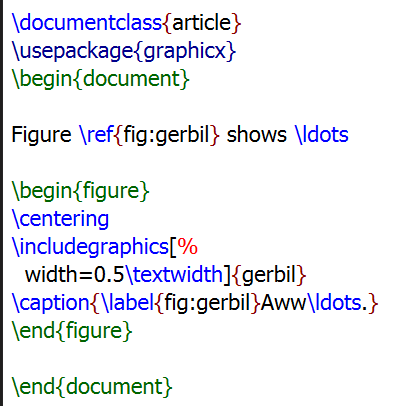
\includegraphics[width=0.5\linewidth]{figs/float_basic.png}
\end{minipage}
\begin{minipage}{0.35\linewidth}
    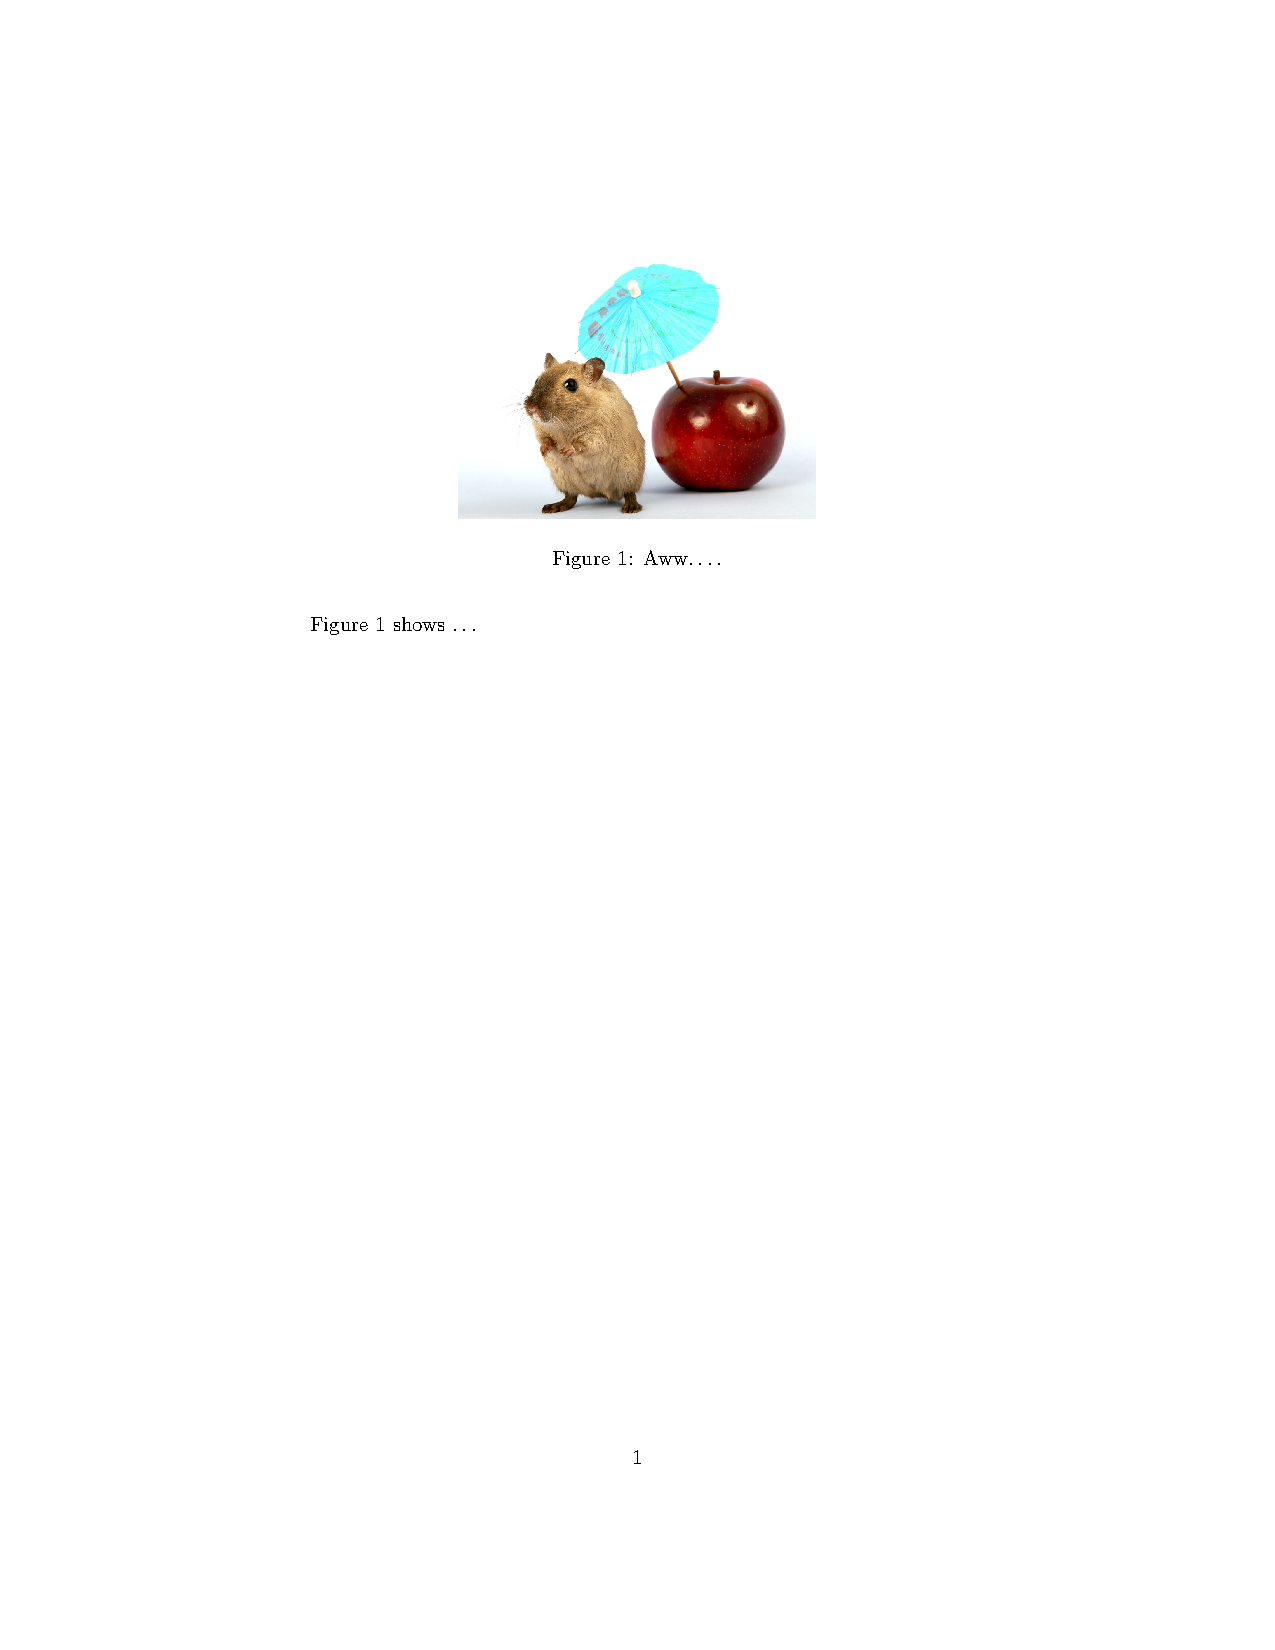
\includegraphics[width=\textwidth,clip,trim=2in 5in 3in 1in]{figs/media-graphics.pdf}
\end{minipage}

\tiny{Image license: \href{https://pixabay.com/en/animal-apple-attractive-beautiful-1239390/}{CC0}}
\end{frame}

%%%%%%%%%%%%%%%%%%%%%%%%%%%%%%%%%%%%%%%%%%%%%%%%%%%%%%%%%%%%%%%%%%%%%%%%%%%%%%%
%%%%%%%%%%%%%%%%%%%%%%%%%%%%%%%%%%%%%%%%%%%%%%%%%%%%%%%%%%%%%%%%%%%%%%%%%%%%%%%
%%%%%%%%%%%%%%%%%%%%%%%%%%%%%%%%%%%%%%%%%%%%%%%%%%%%%%%%%%%%%%%%%%%%%%%%%%%%%%%
\subsection{Tables}
\begin{frame}[fragile]{\insertsubsection}
\begin{itemize}
\item Tables in \LaTeX{} take some getting used to.
\item Use the \bftt{tabular} environment from the \bftt{tabularx} package.
\item The argument specifies column alignment --- \textbf{l}eft, \textbf{r}ight, \textbf{r}ight.
\begin{figure}
    % \centering
    \begin{minipage}{0.5\textwidth}
        \begin{lstlisting}
\begin{tabular}{lrr}
    Item   & Qty & Unit \$ \\
    Widget & 1   & 199.99  \\
    Gadget & 2   & 399.99  \\
    Cable  & 3   & 19.99   \\
\end{tabular}
        \end{lstlisting}
    \end{minipage}
    \begin{minipage}{0.4\textwidth}
        \begin{tabular}{lrr}
        Item   & Qty & Unit \$ \\
        Widget & 1   & 199.99  \\
        Gadget & 2   & 399.99  \\
        Cable  & 3   & 19.99   \\
        \end{tabular}
    \end{minipage}
\end{figure}
\item It also specifies vertical lines; use \cmdbs{hline} for horizontal lines.
\begin{figure}
    % \centering
    \begin{minipage}{0.5\textwidth}
        \begin{lstlisting}
\begin{tabular}{|l|r|r|} \hline
    Item   & Qty & Unit \$ \\\hline
    Widget & 1   & 199.99  \\
    Gadget & 2   & 399.99  \\
    Cable  & 3   & 19.99   \\\hline
\end{tabular}
        \end{lstlisting}
    \end{minipage}
    \begin{minipage}{0.4\textwidth}
        \begin{tabular}{|l|r|r|} \hline
            Item   & Qty & Unit \$ \\\hline
            Widget & 1   & 199.99  \\
            Gadget & 2   & 399.99  \\
            Cable  & 3   & 19.99   \\\hline
        \end{tabular}
    \end{minipage}
\end{figure}
\item Use an ampersand \keystrokebftt{\&} to separate columns and a double backslash \keystrokebftt{\bs}\keystrokebftt{\bs} to start a new row (like in the \bftt{align*} environment that we saw in part 1).
\end{itemize}
\end{frame}

%%%%%%%%%%%%%%%%%%%%%%%%%%%%%%%%%%%%%%%%%%%%%%%%%%%%%%%%%%%%%%%%%%%%%%%%%%%%%%%
%%%%%%%%%%%%%%%%%%%%%%%%%%%%%%%%%%%%%%%%%%%%%%%%%%%%%%%%%%%%%%%%%%%%%%%%%%%%%%%
%%%%%%%%%%%%%%%%%%%%%%%%%%%%%%%%%%%%%%%%%%%%%%%%%%%%%%%%%%%%%%%%%%%%%%%%%%%%%%%
\addtocontents{toc}{\newpage}
\section{Bibliographies}

% %%%%%%%%%%%%%%%%%%%%%%%%%%%%%%%%%%%%%%%%%%%%%%%%%%%%%%%%%%%%%%%%%%%%%%%%%%%%%%%
% %%%%%%%%%%%%%%%%%%%%%%%%%%%%%%%%%%%%%%%%%%%%%%%%%%%%%%%%%%%%%%%%%%%%%%%%%%%%%%%
% %%%%%%%%%%%%%%%%%%%%%%%%%%%%%%%%%%%%%%%%%%%%%%%%%%%%%%%%%%%%%%%%%%%%%%%%%%%%%%%
% \begin{frame}{Outline}
% \begin{multicols}{2}
% \tableofcontents[currentsection]
% \end{multicols}
% \end{frame}

%%%%%%%%%%%%%%%%%%%%%%%%%%%%%%%%%%%%%%%%%%%%%%%%%%%%%%%%%%%%%%%%%%%%%%%%%%%%%%%
%%%%%%%%%%%%%%%%%%%%%%%%%%%%%%%%%%%%%%%%%%%%%%%%%%%%%%%%%%%%%%%%%%%%%%%%%%%%%%%
%%%%%%%%%%%%%%%%%%%%%%%%%%%%%%%%%%%%%%%%%%%%%%%%%%%%%%%%%%%%%%%%%%%%%%%%%%%%%%%
\subsection{bib\TeX}
\begin{frame}[fragile]{\insertsubsection{} 1}
\begin{itemize}
\item Put your references in a \bftt{.bib} file in `bibtex' database format:
% \inputminted[fontsize=\scriptsize,frame=single]{latex}{bib-example.bib}
\begin{lstlisting}
@Article{Jacobson1999Towards,
author = {Van Jacobson},
title = {Towards the Analysis of Massive Multiplayer Online
        Role-Playing Games},
journal = {Journal of Ubiquitous Information},
Month = jun,
Year = 1999,
Volume = 6,
Pages = {75--83}}

@InProceedings{Brooks1997Methodology,
author = {Fredrick P. Brooks and John Kubiatowicz and
        Christos Papadimitriou},
title = {A Methodology for the Study of the
        Location-Identity Split},
booktitle = {Proceedings of OOPSLA},
Month = jun,
Year = 1997}
\end{lstlisting}
\item Most reference managers can export to bibtex format.
\end{itemize}
\end{frame}

%%%%%%%%%%%%%%%%%%%%%%%%%%%%%%%%%%%%%%%%%%%%%%%%%%%%%%%%%%%%%%%%%%%%%%%%%%%%%%%
%%%%%%%%%%%%%%%%%%%%%%%%%%%%%%%%%%%%%%%%%%%%%%%%%%%%%%%%%%%%%%%%%%%%%%%%%%%%%%%
%%%%%%%%%%%%%%%%%%%%%%%%%%%%%%%%%%%%%%%%%%%%%%%%%%%%%%%%%%%%%%%%%%%%%%%%%%%%%%%
\begin{frame}[fragile]{\insertsubsection{} 2}
\begin{itemize}
\item Each entry in the \bftt{.bib} file has a \emph{key} that you can use to
reference it in the document. For example, \bftt{Jacobson1999Towards} is the key for this article:
\begin{lstlisting}
@Article{Jacobson1999Towards,
  author = {Van Jacobson},
  ...
}
\end{lstlisting}
\item It's a good idea to use a key based on the name, year and title.
\item \LaTeX{} can automatically format your in-text citations and generate a
list of references; it knows most standard styles, and you can design your own.
\end{itemize}
\end{frame}

% %%%%%%%%%%%%%%%%%%%%%%%%%%%%%%%%%%%%%%%%%%%%%%%%%%%%%%%%%%%%%%%%%%%%%%%%%%%%%%%
% %%%%%%%%%%%%%%%%%%%%%%%%%%%%%%%%%%%%%%%%%%%%%%%%%%%%%%%%%%%%%%%%%%%%%%%%%%%%%%%
% %%%%%%%%%%%%%%%%%%%%%%%%%%%%%%%%%%%%%%%%%%%%%%%%%%%%%%%%%%%%%%%%%%%%%%%%%%%%%%%
% \begin{frame}[fragile]{\insertsubsection{} 3}
% \begin{itemize}
% \item Use the \bftt{natbib} package\footnote{There is a new package with more
%   features named \bftt{biblatex} but most of the articles templates still use
%   \bftt{natbib}.} with \cmdbs{citet} and \cmdbs{citep}.
% \item Reference \cmdbs{bibliography} at the end, and specify a \cmdbs{bibliographystyle}.
% \end{itemize}
% \begin{minipage}{0.55\linewidth}
% \inputminted[fontsize=\scriptsize,frame=single,resetmargins]{latex}%
%   {bib-example.tex}
% \end{minipage}
% \begin{minipage}{0.35\linewidth}
% \includegraphics[width=\textwidth,clip,trim=1.8in 5in 1.8in 1in]{bib-example.pdf}
% \end{minipage}
% \end{frame}

% %%%%%%%%%%%%%%%%%%%%%%%%%%%%%%%%%%%%%%%%%%%%%%%%%%%%%%%%%%%%%%%%%%%%%%%%%%%%%%%
% %%%%%%%%%%%%%%%%%%%%%%%%%%%%%%%%%%%%%%%%%%%%%%%%%%%%%%%%%%%%%%%%%%%%%%%%%%%%%%%
% %%%%%%%%%%%%%%%%%%%%%%%%%%%%%%%%%%%%%%%%%%%%%%%%%%%%%%%%%%%%%%%%%%%%%%%%%%%%%%%
% \subsection{Exercise}
% \begin{frame}[fragile]{Exercise: Putting it All Together}

% Add an image and a bibliography to the paper from the previous exercise.

% \begin{enumerate}
% \item Download these example files to your computer.

% \begin{center}
% \fbox{\href{\fileuri/gerbil.jpg?dl=1}{Click to download example image}}

% \fbox{\href{\fileuri/bib-exercise.bib?dl=1}{Click to download example bib file}}
% \end{center}

% \item Upload them to Overleaf (use the project menu).

% \end{enumerate}
% \end{frame}

%%%%%%%%%%%%%%%%%%%%%%%%%%%%%%%%%%%%%%%%%%%%%%%%%%%%%%%%%%%%%%%%%%%%%%%%%%%%%%%
%%%%%%%%%%%%%%%%%%%%%%%%%%%%%%%%%%%%%%%%%%%%%%%%%%%%%%%%%%%%%%%%%%%%%%%%%%%%%%%
%%%%%%%%%%%%%%%%%%%%%%%%%%%%%%%%%%%%%%%%%%%%%%%%%%%%%%%%%%%%%%%%%%%%%%%%%%%%%%%
\section{What's Next?}

% %%%%%%%%%%%%%%%%%%%%%%%%%%%%%%%%%%%%%%%%%%%%%%%%%%%%%%%%%%%%%%%%%%%%%%%%%%%%%%%
% %%%%%%%%%%%%%%%%%%%%%%%%%%%%%%%%%%%%%%%%%%%%%%%%%%%%%%%%%%%%%%%%%%%%%%%%%%%%%%%
% %%%%%%%%%%%%%%%%%%%%%%%%%%%%%%%%%%%%%%%%%%%%%%%%%%%%%%%%%%%%%%%%%%%%%%%%%%%%%%%
% \begin{frame}{Outline}
% \begin{multicols}{2}
% \tableofcontents[currentsection]
% \end{multicols}
% \end{frame}

%%%%%%%%%%%%%%%%%%%%%%%%%%%%%%%%%%%%%%%%%%%%%%%%%%%%%%%%%%%%%%%%%%%%%%%%%%%%%%%
%%%%%%%%%%%%%%%%%%%%%%%%%%%%%%%%%%%%%%%%%%%%%%%%%%%%%%%%%%%%%%%%%%%%%%%%%%%%%%%
%%%%%%%%%%%%%%%%%%%%%%%%%%%%%%%%%%%%%%%%%%%%%%%%%%%%%%%%%%%%%%%%%%%%%%%%%%%%%%%
\subsection{More Neat Things}
\begin{frame}[fragile]{\insertsubsection}
\begin{itemize}
\item Add the \cmdbs{tableofcontents} command to generate a table of contents
from the \cmdbs{section} commands.

\item Change the \cmdbs{documentclass} to
\verb|\documentclass{scrartcl}|
or
\verb|\documentclass[12pt]{IEEEtran}|

\item Define your own command for a complicated equation:
\begin{figure}
    % \centering
    \begin{minipage}{0.5\textwidth}
        \begin{lstlisting}          
\newcommand{\rperf}{%
\rho_{\text{perf}}}
$$
\rperf = {\bf c}'{\bf X} + \varepsilon
$$
        \end{lstlisting}
    \end{minipage}
    \begin{minipage}{0.4\textwidth}      
\newcommand{\rperf}{%
\rho_{\text{perf}}}
$$
\rperf = {\bf c}'{\bf X} + \varepsilon
$$
    \end{minipage}
\end{figure}
\end{itemize}
\end{frame}

%%%%%%%%%%%%%%%%%%%%%%%%%%%%%%%%%%%%%%%%%%%%%%%%%%%%%%%%%%%%%%%%%%%%%%%%%%%%%%%
%%%%%%%%%%%%%%%%%%%%%%%%%%%%%%%%%%%%%%%%%%%%%%%%%%%%%%%%%%%%%%%%%%%%%%%%%%%%%%%
%%%%%%%%%%%%%%%%%%%%%%%%%%%%%%%%%%%%%%%%%%%%%%%%%%%%%%%%%%%%%%%%%%%%%%%%%%%%%%%
\subsection{More Neat Packages}
\begin{frame}{\insertsubsection}
\begin{itemize}
\item \bftt{beamer}: for presentations (like this one!)
\item \bftt{todonotes}: comments and TODO management
\item \bftt{tikz}: make amazing graphics
\item \bftt{pgfplots}: create graphs in \LaTeX
\item \bftt{listings}: source code printer for \LaTeX
\item \bftt{spreadtab}: create spreadsheets in \LaTeX
\item \bftt{gchords}, \bftt{guitar}: guitar chords and tabulature
\item \bftt{cwpuzzle}: crossword puzzles
\end{itemize}
See \url{https://www.overleaf.com/latex/examples} and \url{http://texample.net}
for examples of (most of) these packages.
\end{frame}

%%%%%%%%%%%%%%%%%%%%%%%%%%%%%%%%%%%%%%%%%%%%%%%%%%%%%%%%%%%%%%%%%%%%%%%%%%%%%%%
%%%%%%%%%%%%%%%%%%%%%%%%%%%%%%%%%%%%%%%%%%%%%%%%%%%%%%%%%%%%%%%%%%%%%%%%%%%%%%%
%%%%%%%%%%%%%%%%%%%%%%%%%%%%%%%%%%%%%%%%%%%%%%%%%%%%%%%%%%%%%%%%%%%%%%%%%%%%%%%
\subsection{Installing \LaTeX{}}
\begin{frame}{\insertsubsection}
\begin{itemize}
\item To run \LaTeX{} on your own computer, you'll want to use a \LaTeX{}
\emph{distribution}. A distribution includes a \bftt{latex} program
and (typically) several thousand packages.
\begin{itemize}
\item On Windows: \href{http://miktex.org/}{Mik\TeX} or \href{http://tug.org/texlive/}{\TeX Live}
\item On Linux: \href{http://tug.org/texlive/}{\TeX Live}
\item On Mac: \href{http://tug.org/mactex/}{Mac\TeX}
\end{itemize}
\item You'll also want a text editor with \LaTeX{} support. See \url{http://en.wikipedia.org/wiki/Comparison_of_TeX_editors} for a list of (many) options.
\item You'll also have to know more about how \bftt{latex} and its related tools
work --- see the resources on the next slide.
\end{itemize}
\end{frame}

%%%%%%%%%%%%%%%%%%%%%%%%%%%%%%%%%%%%%%%%%%%%%%%%%%%%%%%%%%%%%%%%%%%%%%%%%%%%%%%
%%%%%%%%%%%%%%%%%%%%%%%%%%%%%%%%%%%%%%%%%%%%%%%%%%%%%%%%%%%%%%%%%%%%%%%%%%%%%%%
%%%%%%%%%%%%%%%%%%%%%%%%%%%%%%%%%%%%%%%%%%%%%%%%%%%%%%%%%%%%%%%%%%%%%%%%%%%%%%%
\subsection{Online Resources}
\begin{frame}{\insertsubsection}
\begin{itemize}
\item \href{https://www.overleaf.com/learn}{The Overleaf Learn Wiki} ---
hosts these slides, more tutorials and reference material
\item \href{http://en.wikibooks.org/wiki/LaTeX}{The \LaTeX{} Wikibook} ---
excellent tutorials and reference material.
\item \href{http://tex.stackexchange.com/}{\TeX{} Stack Exchange} --- ask
questions and get excellent answers incredibly quickly
\item \href{http://www.latex-community.org/}{\LaTeX{} Community} --- a large
online forum
\item \href{http://ctan.org/}{Comprehensive \TeX{} Archive Network (CTAN)} ---
over four thousand packages plus documentation
\item Google will usually get you to one of the above.
\end{itemize}
\end{frame}


%%%%%%%%%%%%%%%%%%%%%%%%%%%%%%%%%%%%%%%%%%%%%%%%%%%%%%%%%%%%%%%%%%%%%%%%%%%%%%%
%%%%%%%%%%%%%%%%%%%%%%%%%%%%%%%%%%%%%%%%%%%%%%%%%%%%%%%%%%%%%%%%%%%%%%%%%%%%%%%
%%%%%%%%%%%%%%%%%%%%%%%%%%%%%%%%%%%%%%%%%%%%%%%%%%%%%%%%%%%%%%%%%%%%%%%%%%%%%%%
\begin{frame}
\begin{center}
Thanks, and happy \TeX{}ing!
\end{center}
\end{frame}


% %%%%%%%%%%%%%%%%%%%%%%%%%%%%%%%%%%%%%%%%%%%%%%%%%%%%%%%%%%%%%%%%%%%%%%%%%%%%%%%
% %%%%%%%%%%%%%%%%%%%%%%%%%%%%%%%%%%%%%%%%%%%%%%%%%%%%%%%%%%%%%%%%%%%%%%%%%%%%%%%
% %%%%%%%%%%%%%%%%%%%%%%%%%%%%%%%%%%%%%%%%%%%%%%%%%%%%%%%%%%%%%%%%%%%%%%%%%%%%%%%
% \section{\LaTeX{} Recap}

% %%%%%%%%%%%%%%%%%%%%%%%%%%%%%%%%%%%%%%%%%%%%%%%%%%%%%%%%%%%%%%%%%%%%%%%%%%%%%%%
% %%%%%%%%%%%%%%%%%%%%%%%%%%%%%%%%%%%%%%%%%%%%%%%%%%%%%%%%%%%%%%%%%%%%%%%%%%%%%%%
% %%%%%%%%%%%%%%%%%%%%%%%%%%%%%%%%%%%%%%%%%%%%%%%%%%%%%%%%%%%%%%%%%%%%%%%%%%%%%%%
% \begin{frame}[fragile]{\insertsection}
% \begin{itemize}
% \item You write your document in \texttt{plain text} with \cmd{commands} that
% describe its structure and meaning.
% \item The \texttt{latex} program processes your text and commands to produce a
% beautifully formatted document.
% \end{itemize}
% \vskip 2ex
% \begin{center}
% \begin{minted}[frame=single]{latex}
% The rain in Spain falls \emph{mainly} on the plain.
% \end{minted}
% \vskip 2ex
% \tikz\node[single arrow,fill=gray,font=\ttfamily\bfseries,%
%   rotate=270,xshift=-1em]{latex};
% \vskip 2ex
% \fbox{The rain in Spain falls \emph{mainly} on the plain.}
% \end{center}
% \end{frame}

% %%%%%%%%%%%%%%%%%%%%%%%%%%%%%%%%%%%%%%%%%%%%%%%%%%%%%%%%%%%%%%%%%%%%%%%%%%%%%%%
% %%%%%%%%%%%%%%%%%%%%%%%%%%%%%%%%%%%%%%%%%%%%%%%%%%%%%%%%%%%%%%%%%%%%%%%%%%%%%%%
% %%%%%%%%%%%%%%%%%%%%%%%%%%%%%%%%%%%%%%%%%%%%%%%%%%%%%%%%%%%%%%%%%%%%%%%%%%%%%%%
% \begin{frame}[fragile]{\insertsection: Commands \& Arguments}
% \begin{itemize}
% \item A command starts with a \emph{backslash} \keystrokebftt{\bs}.
% \item Some commands take an \emph{argument} in curly braces \keystrokebftt{\{}
% \keystrokebftt{\}}.
% \item Some commands also take \emph{optional arguments} in square brackets \keystrokebftt{[} \keystrokebftt{]}.
% \vskip 2ex
% \begin{exampletwouptiny}
% \includegraphics[
%   width=0.5\textwidth]{gerbil}

% \includegraphics[
%   width=0.3\textwidth,
%   angle=270]{gerbil}
% \end{exampletwouptiny}
% \end{itemize}

% \tiny{Image license: \href{https://pixabay.com/en/animal-apple-attractive-beautiful-1239390/}{CC0}}
% \end{frame}

% %%%%%%%%%%%%%%%%%%%%%%%%%%%%%%%%%%%%%%%%%%%%%%%%%%%%%%%%%%%%%%%%%%%%%%%%%%%%%%%
% %%%%%%%%%%%%%%%%%%%%%%%%%%%%%%%%%%%%%%%%%%%%%%%%%%%%%%%%%%%%%%%%%%%%%%%%%%%%%%%
% %%%%%%%%%%%%%%%%%%%%%%%%%%%%%%%%%%%%%%%%%%%%%%%%%%%%%%%%%%%%%%%%%%%%%%%%%%%%%%%
% \begin{frame}[fragile]{\insertsection: Environments}
% \begin{itemize}
% \item The \cmdbs{begin} and \cmdbs{end} commands are used to create many
% different environments --- contexts.

% \item The \bftt{itemize} and \bftt{enumerate} environments make lists.
% \vskip 2ex
% \begin{exampletwouptiny}
% \begin{itemize} % for bullet points
% \item Biscuits
% \item Tea
% \end{itemize}

% \begin{enumerate} % for numbers
% \item Biscuits
% \item Tea
% \end{enumerate}
% \end{exampletwouptiny}

% \end{itemize}
% \end{frame}

% %%%%%%%%%%%%%%%%%%%%%%%%%%%%%%%%%%%%%%%%%%%%%%%%%%%%%%%%%%%%%%%%%%%%%%%%%%%%%%%
% %%%%%%%%%%%%%%%%%%%%%%%%%%%%%%%%%%%%%%%%%%%%%%%%%%%%%%%%%%%%%%%%%%%%%%%%%%%%%%%
% %%%%%%%%%%%%%%%%%%%%%%%%%%%%%%%%%%%%%%%%%%%%%%%%%%%%%%%%%%%%%%%%%%%%%%%%%%%%%%%
% \begin{frame}[fragile]{\insertsection: Mathematics}
% \begin{itemize}
% \item The \bftt{equation} environment makes a numbered equation.
% \begin{exampletwouptiny}
% \begin{equation}
%   \sum_{k=1}^{n} \frac{1}{2^k}
% \end{equation}
% \end{exampletwouptiny}
% \vskip 2ex

% \item Use dollar signs \keystrokebftt{\$} to mark mathematics in text.\\[1ex]
% \begin{exampletwouptiny}
% % not so good:
% Let a and b be distinct positive
% integers, and let c = a - b + 1.

% % much better:
% Let $a$ and $b$ be distinct positive
% integers, and let $c = a - b + 1$.
% \end{exampletwouptiny}
% \vskip 2ex
% \item Always use dollar signs in pairs --- one to begin the mathematics, and one
% to end it.
% \vskip 1em
% {\scriptsize In fact, we could have written \bftt{\$...\$} as
% \cmdbegin{math}\bftt{...}\cmdend{math}.}
% \end{itemize}
% \end{frame}

% %%%%%%%%%%%%%%%%%%%%%%%%%%%%%%%%%%%%%%%%%%%%%%%%%%%%%%%%%%%%%%%%%%%%%%%%%%%%%%%
% %%%%%%%%%%%%%%%%%%%%%%%%%%%%%%%%%%%%%%%%%%%%%%%%%%%%%%%%%%%%%%%%%%%%%%%%%%%%%%%
% %%%%%%%%%%%%%%%%%%%%%%%%%%%%%%%%%%%%%%%%%%%%%%%%%%%%%%%%%%%%%%%%%%%%%%%%%%%%%%%
% \begin{frame}[fragile]{\insertsection: Document Structure}
% \begin{itemize}{\small
% \item Starts with the \cmdbs{documentclass} --- what type of document.
% \item Metadata (\cmdbs{title} and \cmdbs{author}) and packages in the
% preamble.
% \item Content between \cmdbegin{document} and \cmdend{document}.
% \item The \cmdbs{maketitle} command creates the title; \cmdbs{section} commands
% create numbered sections.
% }\end{itemize}
% \begin{minipage}{0.55\linewidth}
% \inputminted[fontsize=\scriptsize,frame=single,resetmargins]{latex}%
%   {recap-structure.tex}
% \end{minipage}
% \begin{minipage}{0.35\linewidth}
% % trim: l b r t
% \includegraphics[width=\textwidth,clip,trim=1.5in 7in 3in 2in]{recap-structure.pdf}
% \end{minipage}
% \end{frame}

% %%%%%%%%%%%%%%%%%%%%%%%%%%%%%%%%%%%%%%%%%%%%%%%%%%%%%%%%%%%%%%%%%%%%%%%%%%%%%%%
% %%%%%%%%%%%%%%%%%%%%%%%%%%%%%%%%%%%%%%%%%%%%%%%%%%%%%%%%%%%%%%%%%%%%%%%%%%%%%%%
% %%%%%%%%%%%%%%%%%%%%%%%%%%%%%%%%%%%%%%%%%%%%%%%%%%%%%%%%%%%%%%%%%%%%%%%%%%%%%%%
% \begin{frame}[fragile]{\insertsection: Exercise}

% \begin{enumerate}
% \item Here is the text for a short article:\footnote{Based on \url{http://www.cgd.ucar.edu/cms/agu/scientific_talk.html}}
% \begin{center}
% \fbox{\href{\wlnewdoc{recap-exercise.tex}}{%
% Click to open this exercise in \wllogo{}}}
% \end{center}
% \vskip 2ex
% \item Add \LaTeX{} commands to the text to make it look like this one:
% \begin{center}
% \fbox{\href{\fileuri/recap-exercise-solution.pdf}{%
% Click to open the model document}}
% \end{center}
% \end{enumerate}

% \begin{block}{Hints}
% \begin{itemize}
% \item Use the \bftt{enumerate} and \bftt{itemize} environments for lists.
% \item To typeset a \keystrokebftt{\%} percent sign, \emph{escape} it with a backslash (\cmdbs{\%}).
% \item To typeset the equation, use \cmdbs{frac} for the fraction and the \cmdbs{left(} and \cmdbs{right)} commands for the parentheses.
% \end{itemize}
% \end{block}
% \end{frame}

% %%%%%%%%%%%%%%%%%%%%%%%%%%%%%%%%%%%%%%%%%%%%%%%%%%%%%%%%%%%%%%%%%%%%%%%%%%%%%%%
% %%%%%%%%%%%%%%%%%%%%%%%%%%%%%%%%%%%%%%%%%%%%%%%%%%%%%%%%%%%%%%%%%%%%%%%%%%%%%%%
% %%%%%%%%%%%%%%%%%%%%%%%%%%%%%%%%%%%%%%%%%%%%%%%%%%%%%%%%%%%%%%%%%%%%%%%%%%%%%%%
% \section{Presentations with \protect\bftt{beamer}}

% %%%%%%%%%%%%%%%%%%%%%%%%%%%%%%%%%%%%%%%%%%%%%%%%%%%%%%%%%%%%%%%%%%%%%%%%%%%%%%%
% %%%%%%%%%%%%%%%%%%%%%%%%%%%%%%%%%%%%%%%%%%%%%%%%%%%%%%%%%%%%%%%%%%%%%%%%%%%%%%%
% %%%%%%%%%%%%%%%%%%%%%%%%%%%%%%%%%%%%%%%%%%%%%%%%%%%%%%%%%%%%%%%%%%%%%%%%%%%%%%%
% \begin{frame}[fragile]{\insertsection}
% \begin{itemize}
% \item Beamer is a package for creating presentations (such as this one!) in
% \LaTeX{}.
% \item It provides the \bftt{beamer} document class.
% \item Use the \bftt{frame} environment to create slides.
% \end{itemize}
% \begin{minipage}{0.55\linewidth}
% \inputminted[fontsize=\scriptsize,frame=single,resetmargins]{latex}%
%   {beamer-minimal.tex}
% \end{minipage}
% \begin{minipage}{0.35\linewidth}
% % trim: l b r t
% \includegraphics[width=\textwidth,clip,trim=1in 1in 1in 1in]{beamer-minimal.pdf}
% \end{minipage}
% \end{frame}

% %%%%%%%%%%%%%%%%%%%%%%%%%%%%%%%%%%%%%%%%%%%%%%%%%%%%%%%%%%%%%%%%%%%%%%%%%%%%%%%
% %%%%%%%%%%%%%%%%%%%%%%%%%%%%%%%%%%%%%%%%%%%%%%%%%%%%%%%%%%%%%%%%%%%%%%%%%%%%%%%
% %%%%%%%%%%%%%%%%%%%%%%%%%%%%%%%%%%%%%%%%%%%%%%%%%%%%%%%%%%%%%%%%%%%%%%%%%%%%%%%
% \begin{frame}[fragile]{\insertsection: Following Along}

% \begin{itemize}
% \item As we go through the following slides, try out the examples by typing them
% into the example document on \wllogo.
% \end{itemize}
% \vskip 2ex
% \begin{center}
% \fbox{\href{\wlnewdoc{beamer-minimal.tex}}{%
% Click to open the example document in \wllogo{}}}
% \end{center}
% \end{frame}

% %%%%%%%%%%%%%%%%%%%%%%%%%%%%%%%%%%%%%%%%%%%%%%%%%%%%%%%%%%%%%%%%%%%%%%%%%%%%%%%
% %%%%%%%%%%%%%%%%%%%%%%%%%%%%%%%%%%%%%%%%%%%%%%%%%%%%%%%%%%%%%%%%%%%%%%%%%%%%%%%
% %%%%%%%%%%%%%%%%%%%%%%%%%%%%%%%%%%%%%%%%%%%%%%%%%%%%%%%%%%%%%%%%%%%%%%%%%%%%%%%
% \begin{frame}[fragile]
% \frametitle{\insertsection: Frames}
% \begin{itemize}
% \item Use \cmdbs{frametitle} to give the frame a title.
% \item Then add content to the frame.
% \item The source for this frame looks like:
% \vskip 2ex
% \inputminted[fontsize=\scriptsize,frame=single,resetmargins]{latex}%
%   {beamer-frame.tex}
% \end{itemize}
% \end{frame}

% %%%%%%%%%%%%%%%%%%%%%%%%%%%%%%%%%%%%%%%%%%%%%%%%%%%%%%%%%%%%%%%%%%%%%%%%%%%%%%%
% %%%%%%%%%%%%%%%%%%%%%%%%%%%%%%%%%%%%%%%%%%%%%%%%%%%%%%%%%%%%%%%%%%%%%%%%%%%%%%%
% %%%%%%%%%%%%%%%%%%%%%%%%%%%%%%%%%%%%%%%%%%%%%%%%%%%%%%%%%%%%%%%%%%%%%%%%%%%%%%%
% \begin{frame}[fragile]{\insertsection: Sections}
% \begin{itemize}
% \item You can use \cmdbs{section}s to group your \bftt{frame}s, and
% \bftt{beamer} will use them to create an automatic outline.
% \item To generate an outline, use the \cmdbs{tableofcontents} command. Here's
% one for this presentation. The \bftt{currentsection} option highlights the current section.
% \vskip 2ex
% \begin{exampletwouptiny}
% \tableofcontents[currentsection]
% \end{exampletwouptiny}
% \end{itemize}
% \end{frame}

% %%%%%%%%%%%%%%%%%%%%%%%%%%%%%%%%%%%%%%%%%%%%%%%%%%%%%%%%%%%%%%%%%%%%%%%%%%%%%%%
% %%%%%%%%%%%%%%%%%%%%%%%%%%%%%%%%%%%%%%%%%%%%%%%%%%%%%%%%%%%%%%%%%%%%%%%%%%%%%%%
% %%%%%%%%%%%%%%%%%%%%%%%%%%%%%%%%%%%%%%%%%%%%%%%%%%%%%%%%%%%%%%%%%%%%%%%%%%%%%%%
% \begin{frame}[fragile]{\insertsection: Multiple Columns}
% \begin{columns}
% \begin{column}{0.4\textwidth}
% \begin{itemize}
% \item Use the \bftt{columns} and \bftt{column} environments to break the slide
% into columns.
% \item The argument for each \bftt{column} determines its width.
% \item See also the \bftt{multicol} package, which automatically breaks your
% content into columns.
% \end{itemize}
% \end{column}
% \begin{column}{0.6\textwidth}
% \begin{minted}[fontsize=\scriptsize,frame=single]{latex}
% \begin{columns}
%   \begin{column}{0.4\textwidth}
%     \begin{itemize}
%     \item Use the columns ...
%     \item The argument ...
%     \item See also the ...
%     \end{itemize}
%   \end{column}
%   \begin{column}{0.6\textwidth}
%     % second column
%   \end{column}
% \end{columns}
% \end{minted}
% \end{column}
% \end{columns}
% \end{frame}

% %%%%%%%%%%%%%%%%%%%%%%%%%%%%%%%%%%%%%%%%%%%%%%%%%%%%%%%%%%%%%%%%%%%%%%%%%%%%%%%
% %%%%%%%%%%%%%%%%%%%%%%%%%%%%%%%%%%%%%%%%%%%%%%%%%%%%%%%%%%%%%%%%%%%%%%%%%%%%%%%
% %%%%%%%%%%%%%%%%%%%%%%%%%%%%%%%%%%%%%%%%%%%%%%%%%%%%%%%%%%%%%%%%%%%%%%%%%%%%%%%
% \begin{frame}[fragile]{\insertsection: Highlights}
% \begin{itemize}

% \item Use \cmdbs{emph} or \cmdbs{alert} to highlight:
% \vskip 1ex
% \begin{exampletwouptiny}
% I should \emph{emphasise} that
% this is an \alert{important} point.
% \end{exampletwouptiny}
% \vskip 1ex

% \item Or specify bold face or italics:
% \vskip 1ex
% \begin{exampletwouptiny}
% Text in \textbf{bold face}.
% Text in \textit{italics}.
% \end{exampletwouptiny}
% \vskip 1ex

% \item Or specify a color (American spelling):
% \vskip 1ex
% \begin{exampletwouptiny}
% It \textcolor{red}{stops}
% and \textcolor{green}{starts}.
% \end{exampletwouptiny}
% \vskip 1ex
% \item See \url{http://www.math.umbc.edu/~rouben/beamer/quickstart-Z-H-25.html}
% for more colors \& custom colors.
% \end{itemize}
% \end{frame}

% %%%%%%%%%%%%%%%%%%%%%%%%%%%%%%%%%%%%%%%%%%%%%%%%%%%%%%%%%%%%%%%%%%%%%%%%%%%%%%%
% %%%%%%%%%%%%%%%%%%%%%%%%%%%%%%%%%%%%%%%%%%%%%%%%%%%%%%%%%%%%%%%%%%%%%%%%%%%%%%%
% %%%%%%%%%%%%%%%%%%%%%%%%%%%%%%%%%%%%%%%%%%%%%%%%%%%%%%%%%%%%%%%%%%%%%%%%%%%%%%%
% \begin{frame}[fragile]{\insertsection: Figures}
% \begin{itemize}
% \item Use \cmdbs{includegraphics} from the \bftt{graphicx} package.
% \item The \bftt{figure} environment centers by default, in \bftt{beamer}.
% \vskip 2ex
% \begin{exampletwouptiny}
% \begin{figure}
% \includegraphics[
%   width=0.5\textwidth]{gerbil}
% \end{figure}
% \end{exampletwouptiny}
% \end{itemize}

% \tiny{Image license: \href{https://pixabay.com/en/animal-apple-attractive-beautiful-1239390/}{CC0}}
% \end{frame}

% %%%%%%%%%%%%%%%%%%%%%%%%%%%%%%%%%%%%%%%%%%%%%%%%%%%%%%%%%%%%%%%%%%%%%%%%%%%%%%%
% %%%%%%%%%%%%%%%%%%%%%%%%%%%%%%%%%%%%%%%%%%%%%%%%%%%%%%%%%%%%%%%%%%%%%%%%%%%%%%%
% %%%%%%%%%%%%%%%%%%%%%%%%%%%%%%%%%%%%%%%%%%%%%%%%%%%%%%%%%%%%%%%%%%%%%%%%%%%%%%%
% \begin{frame}[fragile]{\insertsection: Tables}
% \begin{itemize}
% \item Tables in \LaTeX{} take some getting used to.
% \item Use the \bftt{tabular} environment from the \bftt{tabularx} package.
% \item The argument specifies column alignment --- \textbf{l}eft, \textbf{r}ight, \textbf{r}ight.
% \begin{exampletwouptiny}
% \begin{tabular}{lrr}
% Item   & Qty & Unit \$ \\
% Widget & 1   & 199.99  \\
% Gadget & 2   & 399.99  \\
% Cable  & 3   & 19.99   \\
% \end{tabular}
% \end{exampletwouptiny}
% \item It also specifies vertical lines; use \cmdbs{hline} for horizontal lines.
% \begin{exampletwouptiny}
% \begin{tabular}{|l|r|r|} \hline
% Item   & Qty & Unit \$ \\\hline
% Widget & 1   & 199.99  \\
% Gadget & 2   & 399.99  \\
% Cable  & 3   & 19.99   \\\hline
% \end{tabular}
% \end{exampletwouptiny}
% \item Use an ampersand \keystrokebftt{\&} to separate columns and a double backslash \keystrokebftt{\bs}\keystrokebftt{\bs} to start a new row.
% \end{itemize}
% \end{frame}

% %%%%%%%%%%%%%%%%%%%%%%%%%%%%%%%%%%%%%%%%%%%%%%%%%%%%%%%%%%%%%%%%%%%%%%%%%%%%%%%
% %%%%%%%%%%%%%%%%%%%%%%%%%%%%%%%%%%%%%%%%%%%%%%%%%%%%%%%%%%%%%%%%%%%%%%%%%%%%%%%
% %%%%%%%%%%%%%%%%%%%%%%%%%%%%%%%%%%%%%%%%%%%%%%%%%%%%%%%%%%%%%%%%%%%%%%%%%%%%%%%
% \begin{frame}[fragile]{\insertsection: Blocks}
% \begin{itemize}
% \item A \bftt{block} environment makes a titled box.
% \begin{exampletwouptiny}
% \begin{block}{Interesting Fact}
% This is important.
% \end{block}

% \begin{alertblock}{Cautionary Tale}
% This is really important!
% \end{alertblock}
% \end{exampletwouptiny}

% \item How exactly they look depends on the theme\ldots
% \end{itemize}
% \end{frame}

% %%%%%%%%%%%%%%%%%%%%%%%%%%%%%%%%%%%%%%%%%%%%%%%%%%%%%%%%%%%%%%%%%%%%%%%%%%%%%%%
% %%%%%%%%%%%%%%%%%%%%%%%%%%%%%%%%%%%%%%%%%%%%%%%%%%%%%%%%%%%%%%%%%%%%%%%%%%%%%%%
% %%%%%%%%%%%%%%%%%%%%%%%%%%%%%%%%%%%%%%%%%%%%%%%%%%%%%%%%%%%%%%%%%%%%%%%%%%%%%%%
% \begin{frame}[fragile]
% \frametitle{\insertsection: Themes}
% \begin{itemize}
% \item Customise the look of your presentation using themes.
% \item See \url{http://deic.uab.es/~iblanes/beamer_gallery/index_by_theme.html}
% for a large collection of themes.
% \end{itemize}
% \begin{minipage}{0.55\linewidth}
% \inputminted[fontsize=\scriptsize,frame=single,resetmargins]{latex}%
%   {beamer-theme.tex}
% \end{minipage}
% \begin{minipage}{0.35\linewidth}
% % trim: l b r t
% \includegraphics[width=\textwidth]{beamer-theme.pdf}
% \end{minipage}
% \end{frame}

% %%%%%%%%%%%%%%%%%%%%%%%%%%%%%%%%%%%%%%%%%%%%%%%%%%%%%%%%%%%%%%%%%%%%%%%%%%%%%%%
% %%%%%%%%%%%%%%%%%%%%%%%%%%%%%%%%%%%%%%%%%%%%%%%%%%%%%%%%%%%%%%%%%%%%%%%%%%%%%%%
% %%%%%%%%%%%%%%%%%%%%%%%%%%%%%%%%%%%%%%%%%%%%%%%%%%%%%%%%%%%%%%%%%%%%%%%%%%%%%%%
% \begin{frame}[fragile]{\insertsection: Animation}
% \begin{itemize}
% \item A frame can generate multiple slides.
% \item Use the \cmdbs{pause} command to show only part of a slide.
% \vskip 2ex
% \begin{exampletwouptinynoframe}
% \begin{itemize}
% \item Can you feel the 
% \pause \item anticipation?
% \end{itemize}
% \end{exampletwouptinynoframe}
% \vskip 2ex
% \item There many more clever ways of making animations in \bftt{beamer}; see
% also the \cmdbs{only}, \cmdbs{alt}, and \cmdbs{uncover} commands.
% \end{itemize}
% \end{frame}

% %%%%%%%%%%%%%%%%%%%%%%%%%%%%%%%%%%%%%%%%%%%%%%%%%%%%%%%%%%%%%%%%%%%%%%%%%%%%%%%
% %%%%%%%%%%%%%%%%%%%%%%%%%%%%%%%%%%%%%%%%%%%%%%%%%%%%%%%%%%%%%%%%%%%%%%%%%%%%%%%
% %%%%%%%%%%%%%%%%%%%%%%%%%%%%%%%%%%%%%%%%%%%%%%%%%%%%%%%%%%%%%%%%%%%%%%%%%%%%%%%
% \begin{frame}[fragile]{\insertsection: Exercise}

% Recreate Peter Norvig's excellent ``Gettysburg Powerpoint Presentation'' in \bftt{beamer}.\footnote{\url{http://norvig.com/Gettysburg}}

% \begin{enumerate}
% \item Open this exercise in \wllogo{}:
% \begin{center}
% \fbox{\href{\wlnewdoc{beamer-exercise.tex}}{%
% Click to open this exercise in \wllogo{}}}
% \end{center}
% \vskip 2ex
% \item Download this image to your computer and upload it to \wllogo{} via the
% files menu.
% \begin{center}
% \fbox{\href{\fileuri/gettysburg_graph.png?dl=1}{Click to download image}}
% \end{center}
% \vskip 2ex
% \item Add \LaTeX{} commands to the text to make it look like this one:
% \begin{center}
% \fbox{\href{\fileuri/beamer-exercise-solution.pdf}{%
% Click to open the model document}}
% \end{center}
% \end{enumerate}
% \end{frame}

% %%%%%%%%%%%%%%%%%%%%%%%%%%%%%%%%%%%%%%%%%%%%%%%%%%%%%%%%%%%%%%%%%%%%%%%%%%%%%%%
% %%%%%%%%%%%%%%%%%%%%%%%%%%%%%%%%%%%%%%%%%%%%%%%%%%%%%%%%%%%%%%%%%%%%%%%%%%%%%%%
% %%%%%%%%%%%%%%%%%%%%%%%%%%%%%%%%%%%%%%%%%%%%%%%%%%%%%%%%%%%%%%%%%%%%%%%%%%%%%%%
% \section{Drawings with \protect\tikzname}

% %%%%%%%%%%%%%%%%%%%%%%%%%%%%%%%%%%%%%%%%%%%%%%%%%%%%%%%%%%%%%%%%%%%%%%%%%%%%%%%
% %%%%%%%%%%%%%%%%%%%%%%%%%%%%%%%%%%%%%%%%%%%%%%%%%%%%%%%%%%%%%%%%%%%%%%%%%%%%%%%
% %%%%%%%%%%%%%%%%%%%%%%%%%%%%%%%%%%%%%%%%%%%%%%%%%%%%%%%%%%%%%%%%%%%%%%%%%%%%%%%
% \begin{frame}[fragile]{\insertsection}
% \begin{itemize}
% \item \tikzname{} is a package for drawing figures in \LaTeX.
% \item It defines a powerful drawing language inside \LaTeX{}. Short programs can
% draw surprisingly complicated things.
% \begin{figure}
% \href{http://www.texample.net/tikz/examples/rotated-triangle/}{%
%   \includegraphics[width=0.35\textwidth]{rotated-triangle}}
% \end{figure}
% \item We'll start with simple things. To draw a line in \tikzname:
% \vskip 1ex
% \begin{exampletwouptiny}
% \begin{tikzpicture}
% \draw (0,0) -- (1,1); % a line
% \end{tikzpicture}
% \end{exampletwouptiny}
% \end{itemize}
% \end{frame}

% %%%%%%%%%%%%%%%%%%%%%%%%%%%%%%%%%%%%%%%%%%%%%%%%%%%%%%%%%%%%%%%%%%%%%%%%%%%%%%%
% %%%%%%%%%%%%%%%%%%%%%%%%%%%%%%%%%%%%%%%%%%%%%%%%%%%%%%%%%%%%%%%%%%%%%%%%%%%%%%%
% %%%%%%%%%%%%%%%%%%%%%%%%%%%%%%%%%%%%%%%%%%%%%%%%%%%%%%%%%%%%%%%%%%%%%%%%%%%%%%%
% \begin{frame}[fragile]{\insertsection: Coordinates}
% \begin{itemize}
% \item The default coordinates are centimeters, with the usual sense: 
% \begin{figure}
% \begin{tikzpicture}[scale=0.5]
% \draw[help lines] (0,0) grid (3,3);
% \node[below left] at (0,0) {$(0,0)$};
% \node[below right] at (3,0) {$(3,0)$};
% \node[above right] at (3,3) {$(3,3)$};
% \node[above left] at (0,3) {$(0,3)$};
% \end{tikzpicture}
% \end{figure}
% \item It helps to draw a grid when you are working with \tikzname:
% \vskip 1ex
% \begin{exampletwouptiny}
% \begin{tikzpicture}
% \draw[help lines] (0,0) grid (3,3);
% \end{tikzpicture}
% \end{exampletwouptiny}
% \end{itemize}
% \end{frame}

% %%%%%%%%%%%%%%%%%%%%%%%%%%%%%%%%%%%%%%%%%%%%%%%%%%%%%%%%%%%%%%%%%%%%%%%%%%%%%%%
% %%%%%%%%%%%%%%%%%%%%%%%%%%%%%%%%%%%%%%%%%%%%%%%%%%%%%%%%%%%%%%%%%%%%%%%%%%%%%%%
% %%%%%%%%%%%%%%%%%%%%%%%%%%%%%%%%%%%%%%%%%%%%%%%%%%%%%%%%%%%%%%%%%%%%%%%%%%%%%%%
% \begin{frame}[fragile]{\insertsection: Lines}
% \begin{itemize}
% \item Arrow heads and line styles are specified as options to the \cmdbs{draw} command.
% \item End each draw command with a \keystrokebftt{;} semicolon.
% \vskip 1ex
% \begin{exampletwouptiny}
% \begin{tikzpicture}
% \draw[help lines] (0,0) grid (3,3);
% \draw[->] (0,0) -- (1,1);
% \draw[<->, thick] (2,1) -- (1,2);
% \draw[<-, thick, dashed] (2,2)--(3,3);
% \end{tikzpicture}
% \end{exampletwouptiny}
% \end{itemize}
% \end{frame}

% %%%%%%%%%%%%%%%%%%%%%%%%%%%%%%%%%%%%%%%%%%%%%%%%%%%%%%%%%%%%%%%%%%%%%%%%%%%%%%%
% %%%%%%%%%%%%%%%%%%%%%%%%%%%%%%%%%%%%%%%%%%%%%%%%%%%%%%%%%%%%%%%%%%%%%%%%%%%%%%%
% %%%%%%%%%%%%%%%%%%%%%%%%%%%%%%%%%%%%%%%%%%%%%%%%%%%%%%%%%%%%%%%%%%%%%%%%%%%%%%%
% \begin{frame}[fragile]{\insertsection: Paths}
% \begin{itemize}
% \item You can specify multiple points to form a path.
% \item Arrows will appear only at the ends of the path.
% \vskip 1ex
% \begin{exampletwouptiny}
% \begin{tikzpicture}
% \draw[help lines] (0,0) grid (3,3);
% % axes:
% \draw[<->, thick] (0,3)--(0,0)--(3,0);
% % diamond:
% \draw (1.5,0.5) -- (2.5,1.5) -- 
%       (1.5,2.5) -- (0.5,1.5) --
%       cycle; % close the path
% \end{tikzpicture}
% \end{exampletwouptiny}
% \end{itemize}
% \end{frame}

% %%%%%%%%%%%%%%%%%%%%%%%%%%%%%%%%%%%%%%%%%%%%%%%%%%%%%%%%%%%%%%%%%%%%%%%%%%%%%%%
% %%%%%%%%%%%%%%%%%%%%%%%%%%%%%%%%%%%%%%%%%%%%%%%%%%%%%%%%%%%%%%%%%%%%%%%%%%%%%%%
% %%%%%%%%%%%%%%%%%%%%%%%%%%%%%%%%%%%%%%%%%%%%%%%%%%%%%%%%%%%%%%%%%%%%%%%%%%%%%%%
% \begin{frame}[fragile]{\insertsection: Colours}
% \begin{itemize}
% \item Colours are also specified as options to \cmdbs{draw}.
% \vskip 1ex
% \begin{exampletwouptiny}
% \begin{tikzpicture}
% \draw[help lines] (0,0) grid (3,3);
% % axes
% \draw[<->, thick, red]
%   (0,3)--(0,0)--(3,0); 
% % diamond
% \draw[thick, blue, fill=yellow]
%   (1.5,0.5) -- (2.5,1.5) -- 
%   (1.5,2.5) -- (0.5,1.5) --
%   cycle;
% \end{tikzpicture}
% \end{exampletwouptiny}
% \end{itemize}
% \end{frame}

% %%%%%%%%%%%%%%%%%%%%%%%%%%%%%%%%%%%%%%%%%%%%%%%%%%%%%%%%%%%%%%%%%%%%%%%%%%%%%%%
% %%%%%%%%%%%%%%%%%%%%%%%%%%%%%%%%%%%%%%%%%%%%%%%%%%%%%%%%%%%%%%%%%%%%%%%%%%%%%%%
% %%%%%%%%%%%%%%%%%%%%%%%%%%%%%%%%%%%%%%%%%%%%%%%%%%%%%%%%%%%%%%%%%%%%%%%%%%%%%%%
% \begin{frame}[fragile]{\insertsection: Shapes}
% \begin{itemize}
% \item \tikzname{} has built-in commands for simple shapes.
% \vskip 1ex
% \begin{exampletwouptiny}
% \begin{tikzpicture}
% \draw[help lines] (0,0) grid (3,3);
% \draw (1.5,2.0) circle (0.5);
% \draw (0.5,0.5) rectangle (2.5,1.5);
% \end{tikzpicture}
% \end{exampletwouptiny}
% \end{itemize}
% \end{frame}

% %%%%%%%%%%%%%%%%%%%%%%%%%%%%%%%%%%%%%%%%%%%%%%%%%%%%%%%%%%%%%%%%%%%%%%%%%%%%%%%
% %%%%%%%%%%%%%%%%%%%%%%%%%%%%%%%%%%%%%%%%%%%%%%%%%%%%%%%%%%%%%%%%%%%%%%%%%%%%%%%
% %%%%%%%%%%%%%%%%%%%%%%%%%%%%%%%%%%%%%%%%%%%%%%%%%%%%%%%%%%%%%%%%%%%%%%%%%%%%%%%
% \begin{frame}[fragile]{\insertsection: Nodes \& Labels}
% \begin{itemize}
% \item Use nodes to place text (and math) in \tikzname{} drawings.
% \item You can also use nodes as coordinates --- useful for diagrams.
% \vskip 1ex
% \begin{exampletwouptiny}
% \begin{tikzpicture}
% \draw[help lines] (0,0) grid (3,3);
% \node (h) at (0,0) {H};
% \node (x) at (1.5,1.5) {$\xi$};
% \node (t) at (3,0) {T};
% \draw[->] (x) -- (h);
% \draw[->] (x) -- (t);
% \end{tikzpicture}
% \end{exampletwouptiny}
% \end{itemize}
% \end{frame}

% %%%%%%%%%%%%%%%%%%%%%%%%%%%%%%%%%%%%%%%%%%%%%%%%%%%%%%%%%%%%%%%%%%%%%%%%%%%%%%%
% %%%%%%%%%%%%%%%%%%%%%%%%%%%%%%%%%%%%%%%%%%%%%%%%%%%%%%%%%%%%%%%%%%%%%%%%%%%%%%%
% %%%%%%%%%%%%%%%%%%%%%%%%%%%%%%%%%%%%%%%%%%%%%%%%%%%%%%%%%%%%%%%%%%%%%%%%%%%%%%%
% \begin{frame}[fragile]{\insertsection: Functions}
% \begin{itemize}
% \item You can even plot some simple functions.
% \vskip 1ex
% \begin{exampletwouptiny}
% \begin{tikzpicture}[scale=0.5]
% % y axis
% \draw[<->, thick] (0,2) -- (0,-2);
% % x axis
% \draw[ ->, thick] (0,0) -- (7, 0); 
% % curves
% \draw[cyan,domain=0:2*pi]
%   plot (\x, {sin(\x r)});
% \draw[magenta,domain=0:2*pi]
%   plot (\x, {cos(\x r)});
% \end{tikzpicture}
% \end{exampletwouptiny}
% \end{itemize}
% \end{frame}

% %%%%%%%%%%%%%%%%%%%%%%%%%%%%%%%%%%%%%%%%%%%%%%%%%%%%%%%%%%%%%%%%%%%%%%%%%%%%%%%
% %%%%%%%%%%%%%%%%%%%%%%%%%%%%%%%%%%%%%%%%%%%%%%%%%%%%%%%%%%%%%%%%%%%%%%%%%%%%%%%
% %%%%%%%%%%%%%%%%%%%%%%%%%%%%%%%%%%%%%%%%%%%%%%%%%%%%%%%%%%%%%%%%%%%%%%%%%%%%%%%
% \begin{frame}[fragile]{\insertsection: Examples}
% \begin{itemize}
% \item Check out \fbox{\href{http://texample.net/tikz/}{\TeX{}ample.net}} for many \tikzname{} examples:
% \end{itemize}
% \begin{figure}
% \href{http://texample.net/tikz/examples/escher-brick-penrose-triangle/}{%
%   \includegraphics[width=0.3\textwidth]{escher-brick-penrose-triangle}}
% \href{http://texample.net/tikz/examples/computer-science-mindmap/}{%
%   \includegraphics[width=0.3\textwidth]{computer-science-mindmap}}
% \href{http://texample.net/tikz/examples/gajski-kuhn-y-chart/}{%
%   \includegraphics[width=0.3\textwidth]{gajski-kuhn-y-chart}}
% \end{figure}
% \end{frame}

% %%%%%%%%%%%%%%%%%%%%%%%%%%%%%%%%%%%%%%%%%%%%%%%%%%%%%%%%%%%%%%%%%%%%%%%%%%%%%%%
% %%%%%%%%%%%%%%%%%%%%%%%%%%%%%%%%%%%%%%%%%%%%%%%%%%%%%%%%%%%%%%%%%%%%%%%%%%%%%%%
% %%%%%%%%%%%%%%%%%%%%%%%%%%%%%%%%%%%%%%%%%%%%%%%%%%%%%%%%%%%%%%%%%%%%%%%%%%%%%%%
% \begin{frame}[fragile]{\insertsection: Exercise}
% Draw this in \tikzname:\footnote{Based on \url{http://xkcd.com/1022}}
% \begin{figure}
% \input{tikz-exercise-solution}
% \end{figure}
% \end{frame}

% %%%%%%%%%%%%%%%%%%%%%%%%%%%%%%%%%%%%%%%%%%%%%%%%%%%%%%%%%%%%%%%%%%%%%%%%%%%%%%%
% %%%%%%%%%%%%%%%%%%%%%%%%%%%%%%%%%%%%%%%%%%%%%%%%%%%%%%%%%%%%%%%%%%%%%%%%%%%%%%%
% %%%%%%%%%%%%%%%%%%%%%%%%%%%%%%%%%%%%%%%%%%%%%%%%%%%%%%%%%%%%%%%%%%%%%%%%%%%%%%%
% \section{Notes with \protect\bftt{todonotes}}

% %%%%%%%%%%%%%%%%%%%%%%%%%%%%%%%%%%%%%%%%%%%%%%%%%%%%%%%%%%%%%%%%%%%%%%%%%%%%%%%
% %%%%%%%%%%%%%%%%%%%%%%%%%%%%%%%%%%%%%%%%%%%%%%%%%%%%%%%%%%%%%%%%%%%%%%%%%%%%%%%
% %%%%%%%%%%%%%%%%%%%%%%%%%%%%%%%%%%%%%%%%%%%%%%%%%%%%%%%%%%%%%%%%%%%%%%%%%%%%%%%
% \begin{frame}[fragile]{\insertsection}
% \begin{itemize}
% \item The \cmdbs{todo} command from the \bftt{todonotes} package is great for
% leaving notes to yourself and your collaborators.
% \begin{exampletwouptiny}
% \todo{add results}
% \todo[color=blue!20]{fix method}
% \end{exampletwouptiny}
% \vskip 2ex
% \item Pro Tip: define your own commands with \cmdbs{newcommand}
% \begin{minted}[fontsize=\scriptsize,frame=single]{latex}
% \newcommand{\alice}[1]{\todo[color=green!40]{#1}}
% \newcommand{\bob}[1]{\todo[color=purple!40]{#1}}
% \end{minted}
% This can save a lot of typing:
% \begin{exampletwouptiny}
% \alice{add results}
% \bob{fix method}
% \end{exampletwouptiny}
% \end{itemize}
% \end{frame}

% %%%%%%%%%%%%%%%%%%%%%%%%%%%%%%%%%%%%%%%%%%%%%%%%%%%%%%%%%%%%%%%%%%%%%%%%%%%%%%%
% %%%%%%%%%%%%%%%%%%%%%%%%%%%%%%%%%%%%%%%%%%%%%%%%%%%%%%%%%%%%%%%%%%%%%%%%%%%%%%%
% %%%%%%%%%%%%%%%%%%%%%%%%%%%%%%%%%%%%%%%%%%%%%%%%%%%%%%%%%%%%%%%%%%%%%%%%%%%%%%%
% \begin{frame}[fragile]{\insertsection}
% \begin{columns}
%   \begin{column}{0.4\textwidth}
%     \begin{itemize}
%     \item Only inline notes are supported with beamer, but margin notes are
%     supported for normal documents.
%     \item There is also a handy \cmdbs{listoftodos} command.
%     \end{itemize}
%   \end{column}
%   \begin{column}{0.6\textwidth}
%     \includegraphics[width=\textwidth,page=1]{todonotes-example}
%   \end{column}
% \end{columns}
% \end{frame}

% %%%%%%%%%%%%%%%%%%%%%%%%%%%%%%%%%%%%%%%%%%%%%%%%%%%%%%%%%%%%%%%%%%%%%%%%%%%%%%%
% %%%%%%%%%%%%%%%%%%%%%%%%%%%%%%%%%%%%%%%%%%%%%%%%%%%%%%%%%%%%%%%%%%%%%%%%%%%%%%%
% %%%%%%%%%%%%%%%%%%%%%%%%%%%%%%%%%%%%%%%%%%%%%%%%%%%%%%%%%%%%%%%%%%%%%%%%%%%%%%%
% \section{Spreadsheets with \protect\bftt{spreadtab}}

% %%%%%%%%%%%%%%%%%%%%%%%%%%%%%%%%%%%%%%%%%%%%%%%%%%%%%%%%%%%%%%%%%%%%%%%%%%%%%%%
% %%%%%%%%%%%%%%%%%%%%%%%%%%%%%%%%%%%%%%%%%%%%%%%%%%%%%%%%%%%%%%%%%%%%%%%%%%%%%%%
% %%%%%%%%%%%%%%%%%%%%%%%%%%%%%%%%%%%%%%%%%%%%%%%%%%%%%%%%%%%%%%%%%%%%%%%%%%%%%%%
% \begin{frame}[fragile]{\insertsection}
% \begin{itemize}
% \item Now that you've seen how \LaTeX{} can replace Word and PowerPoint, what
% about Excel?
% \item Homework: try the \fbox{\href{http://www.ctan.org/pkg/spreadtab}{\bftt{spreadtab} package}}!
% \end{itemize}
% \end{frame}

% %%%%%%%%%%%%%%%%%%%%%%%%%%%%%%%%%%%%%%%%%%%%%%%%%%%%%%%%%%%%%%%%%%%%%%%%%%%%%%%
% %%%%%%%%%%%%%%%%%%%%%%%%%%%%%%%%%%%%%%%%%%%%%%%%%%%%%%%%%%%%%%%%%%%%%%%%%%%%%%%
% %%%%%%%%%%%%%%%%%%%%%%%%%%%%%%%%%%%%%%%%%%%%%%%%%%%%%%%%%%%%%%%%%%%%%%%%%%%%%%%
% \begin{frame}
% \begin{center}
% Thanks, and happy \TeX{}ing!
% \end{center}
% \end{frame}

\end{document}